\documentclass{article}
\usepackage[english,polish]{babel}
\selectlanguage{polish}

\title{\huge  \Huge \textbf{MOZA Projekt} \\ \textbf{Wzmacniacz Kaskodowy 4 (wariant B)}}
\date{\today}
\author{ \LARGE Jakub Półtorak}

\usepackage{amsmath}
\usepackage{amsfonts}
\usepackage{graphicx}
\usepackage[T1]{fontenc}
\usepackage{pdflscape}
\usepackage{rotating}
\usepackage[hidelinks]{hyperref}

\begin{document}
\maketitle
\pagenumbering{gobble}
\newpage
\pagenumbering{arabic}
\tableofcontents

\pagebreak

\begin{center}
    \title{ \huge \textbf{Etap 1}}
    \addcontentsline{toc}{section}{Etap 1}
    \label{sec:Etap 1}

\end{center}

\section*{Opis problemu}
Zadanie polega na doborze wartości elementów wzmacniacza tak, aby uzyskać maksymalnie duży iloczyn
GBW. Na układ nałożono dodatkowe ograniczenia w postaci minimalnego wzmocnienia dla małych częstotliwości $k_{u0} > 20 dB$ ($10 \frac{V}{V}$ dla źródła AC o amplitudzie 1 V) oraz minimalnej częstotliwości
granicznej $f_g > 200 MHz$ (rozumianej jako częstotliwość spadku o 3 dB względem $k_{u0}$).

Scheamt wzmacniacza przedstawia poniższy rysunek:
\begin{figure}[h]
    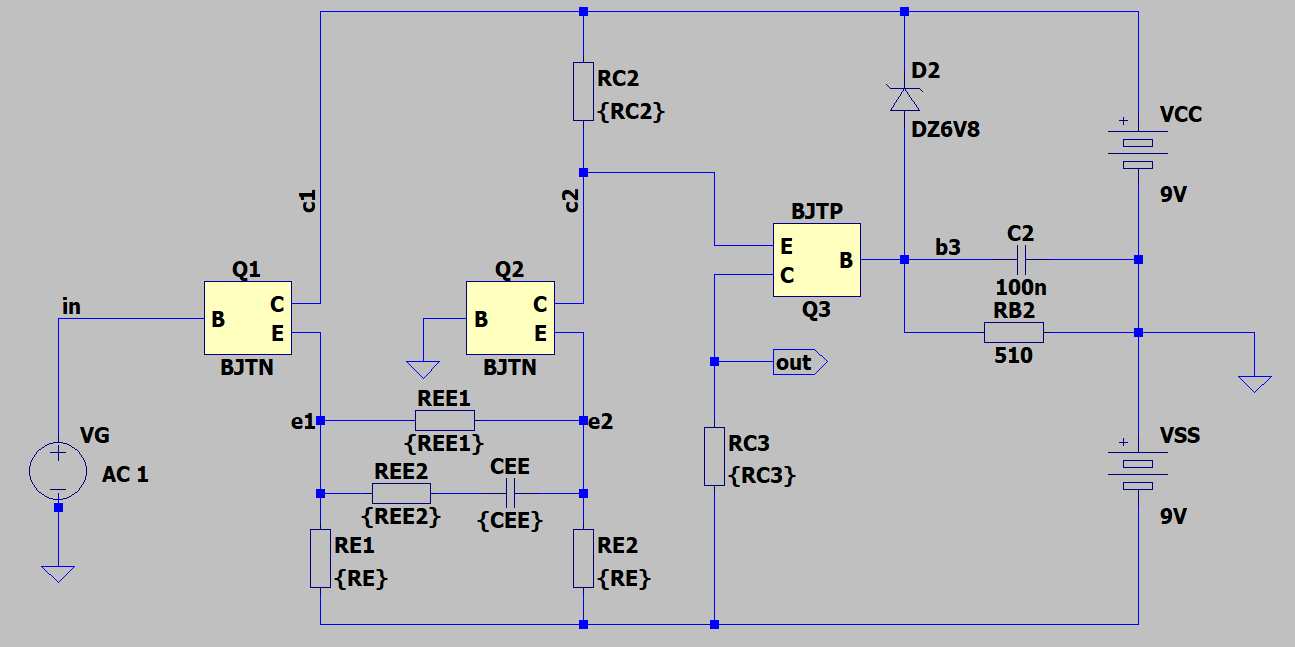
\includegraphics[width=12cm]{graphics/KASK4.png}
    \centering
    \caption{Schemat optymalizowanego układu.}
\end{figure}

\section{Sformułowanie matematyczne zadania optymalizacji}

\subsection{Optymalizacja jednokryterialna}
Poszukiwane jest minimum funkcji celu:
\[ \min\limits_{\textbf{x}\in \mathbf{R}^+  } f(\textbf{x}) \]
p.o.
\[ g_{i}(\textbf{x}) \leq 0 \ \ \ \  i=1..n_g\]
gdzie:
\[ f(\textbf{x}) = -(k_{u0}\cdot f_g)\]
\(\textbf{x}\) - wektor zmiennych optymalizowanych: \\
\begin{center}
    $\textbf{x}$ =
    $\begin{bmatrix}
            REE1 & REE2 & RE & RC2 & RC3 & CEE & CG
        \end{bmatrix}$,
\end{center}
\(k_{u0}(\textbf{x}) [dB]\) - wzmocnienie dla małych częstotliwości, rozumiane jako wzmocnienie dla częstotliwości 1 kHz. \textbf{Ponieważ w symulatorze LTSPICE do symulacji AC wykrozstywane jest źródło AC o amplitudzie 1V zmieniono zapis ograniczenia ( i wszytskich inforamcji
dot $k_u$ z jednostki $\frac{V}{V}$ na dB. Wymagane wzmocnienie $10\frac{V}{V} jest równe 20 dB$)}\\
\(f_{g}(\textbf{x}) [Hz]\) - częstotliwość graniczna, rozumiana jako częstotliwość, dla której wzmocnienie
spada o 3 dB względem $k_{u_{0}}(\textbf{x}) $.

Parametry $k_{u0}(\textbf{x})$ oraz $f_g(\textbf{x})$ obliczane są w Matlabie na podstawie surowych danych ($U^{AC}_{out}(x,f)$) zwracanych
przez symulator LTSpice.

Dodatkowo, w zadaniu pojawiają się ograniczenia nieliniowe związane z wymaganiami projektowymi:\\
\begin{itemize}
    \item \(g_1(\textbf{x}): -(\frac{k_{u0}(\textbf{x})}{k_{u_{min}}}-1) <  0\) \\ Warunek minimalnego wzmocnienia, $k_{umin}=20dB$
    \item \(g_2(\textbf{x}): -(\frac{{f_g}(\textbf{x})}{f_{g_{min}}}-1)<0\) \\ Warunek minimalnej częstotliwości granicznej, $f_{gmin}=200 MHz$. Częstotliwość graniczna $f_g$ obliczana jest jako częstotliwość,
          dla której wzmocnienie spada o 3 dB względem $ku_0$.
    \item \(g_3(\textbf{x}): b(\textbf{x})-b_{max}<0\) \\ Ograniczenie podbicia charakterystyki, $b_{max}=1dB$. Podbicie $b(\textbf{x})$ rozumiane jest jako różnica między maksymalnym poziomem wzmocnienia a $k_{u0}$ ((czyli $b(\textbf{x})=max(k_{u}(\textbf{x}))-b_{max}$)).Podbicie jest obliczane w Matlabie.

\end{itemize}
\subsection{Optymalizacja wielokryterialna}
Poszukiwane jest minimum funkcji celu:
\[ \min\limits_{\textbf{x}\in \mathbf{R}^+  } [f_1(\textbf{x}), f_2(\textbf{x})] \]
p.o.
\[ g_{i}(\textbf{x}) \leq 0 \ \ \ \  i=1..n_g\]
gdzie:
\[ f_1(\textbf{x}) = -k_{u0} [dB]\] \[ f_2(\textbf{x}) = -f_g [Hz]\]
\(\textbf{x}\) - wektor zmiennych optymalizowanych: \\
\begin{center}
    $\textbf{x}$ =
    $\begin{bmatrix}
            REE1 & REE2 & RE & RC2 & RC3 & CEE & CG
        \end{bmatrix}$,
\end{center}
\(k_{u0}(\textbf{x})\) - wzmocnienie dla małych częstotliwości, rozumiane jako wzmocnienie dla częstotliwości 1 kHz.\\
\(f_{g}(\textbf{x})\) - częstotliwość graniczna, rozumiana jako częstotliwość, dla której wzmocnienie
spada o 3 dB względem $k_{u_{0}}(\textbf{x}) $.

Parametry $k_{u0}(\textbf{x})$ oraz $f_g(\textbf{x})$ obliczane są w Matlabie na podstawie surowych danych ($U^{AC}_{out}(x,f)$) zwracanych
przez symulator LTSpice.

Dodatkowo, w zadaniu pojawiają się ograniczenia nieliniowe związane z wymaganiami projektowymi (identyczne jak dla optymalizacji jednokryterialnej):\\
\begin{itemize}
    \item \(g_1(\textbf{x}): -(\frac{k_{u0}(\textbf{x})}{k_{u_{min}}}-1) <  0\) \\ Warunek minimalnego wzmocnienia, $k_{umin}=20dB$
    \item \(g_2(\textbf{x}): -(\frac{{f_g}(\textbf{x})}{f_{g_{min}}}-1)<0\) \\ Warunek minimalnej częstotliwości granicznej, $f_{gmin}=200 MHz$. Częstotliwość graniczna $f_g$ obliczana jest jako częstotliwość,
          dla której wzmocnienie spada o 3 dB względem $ku_0$.
    \item \(g_3(\textbf{x}): b(\textbf{x})-b_{max}<0\) \\ Ograniczenie podbicia charakterystyki, $b_{max}=1dB$. Podbicie $b(\textbf{x})$ rozumiane jest jako różnica między maksymalnym poziomem wzmocnienia a $k_{u0}$ ((czyli $b(\textbf{x})=max(k_{u}(\textbf{x}))-b_{max}$)).Podbicie jest obliczane w Matlabie.

\end{itemize}



\section{Wyznaczenie przybliżenia początkowego rozwiązania}
Zgodnie z poleceniem zmodyfikowano domyślne wartości elementów tak, aby uzyskać rozwiązanie spełniające warunek minimalnej częstotliwości granicznej i wzmocnienia.
Ostatecznie, po wybraniu wartości, wektor \textbf{x} wygląda następująco:
\begin{center}
    $\textbf{x}$ =
    $\begin{bmatrix}
            5\Omega & 15\Omega & 320\Omega & 220\Omega & 200\Omega & 45p & 50p
        \end{bmatrix}$,
\end{center}

Wyniki w punkcie początkowym można zobaczyć na poniższym wykresie:

\begin{figure}[h]
    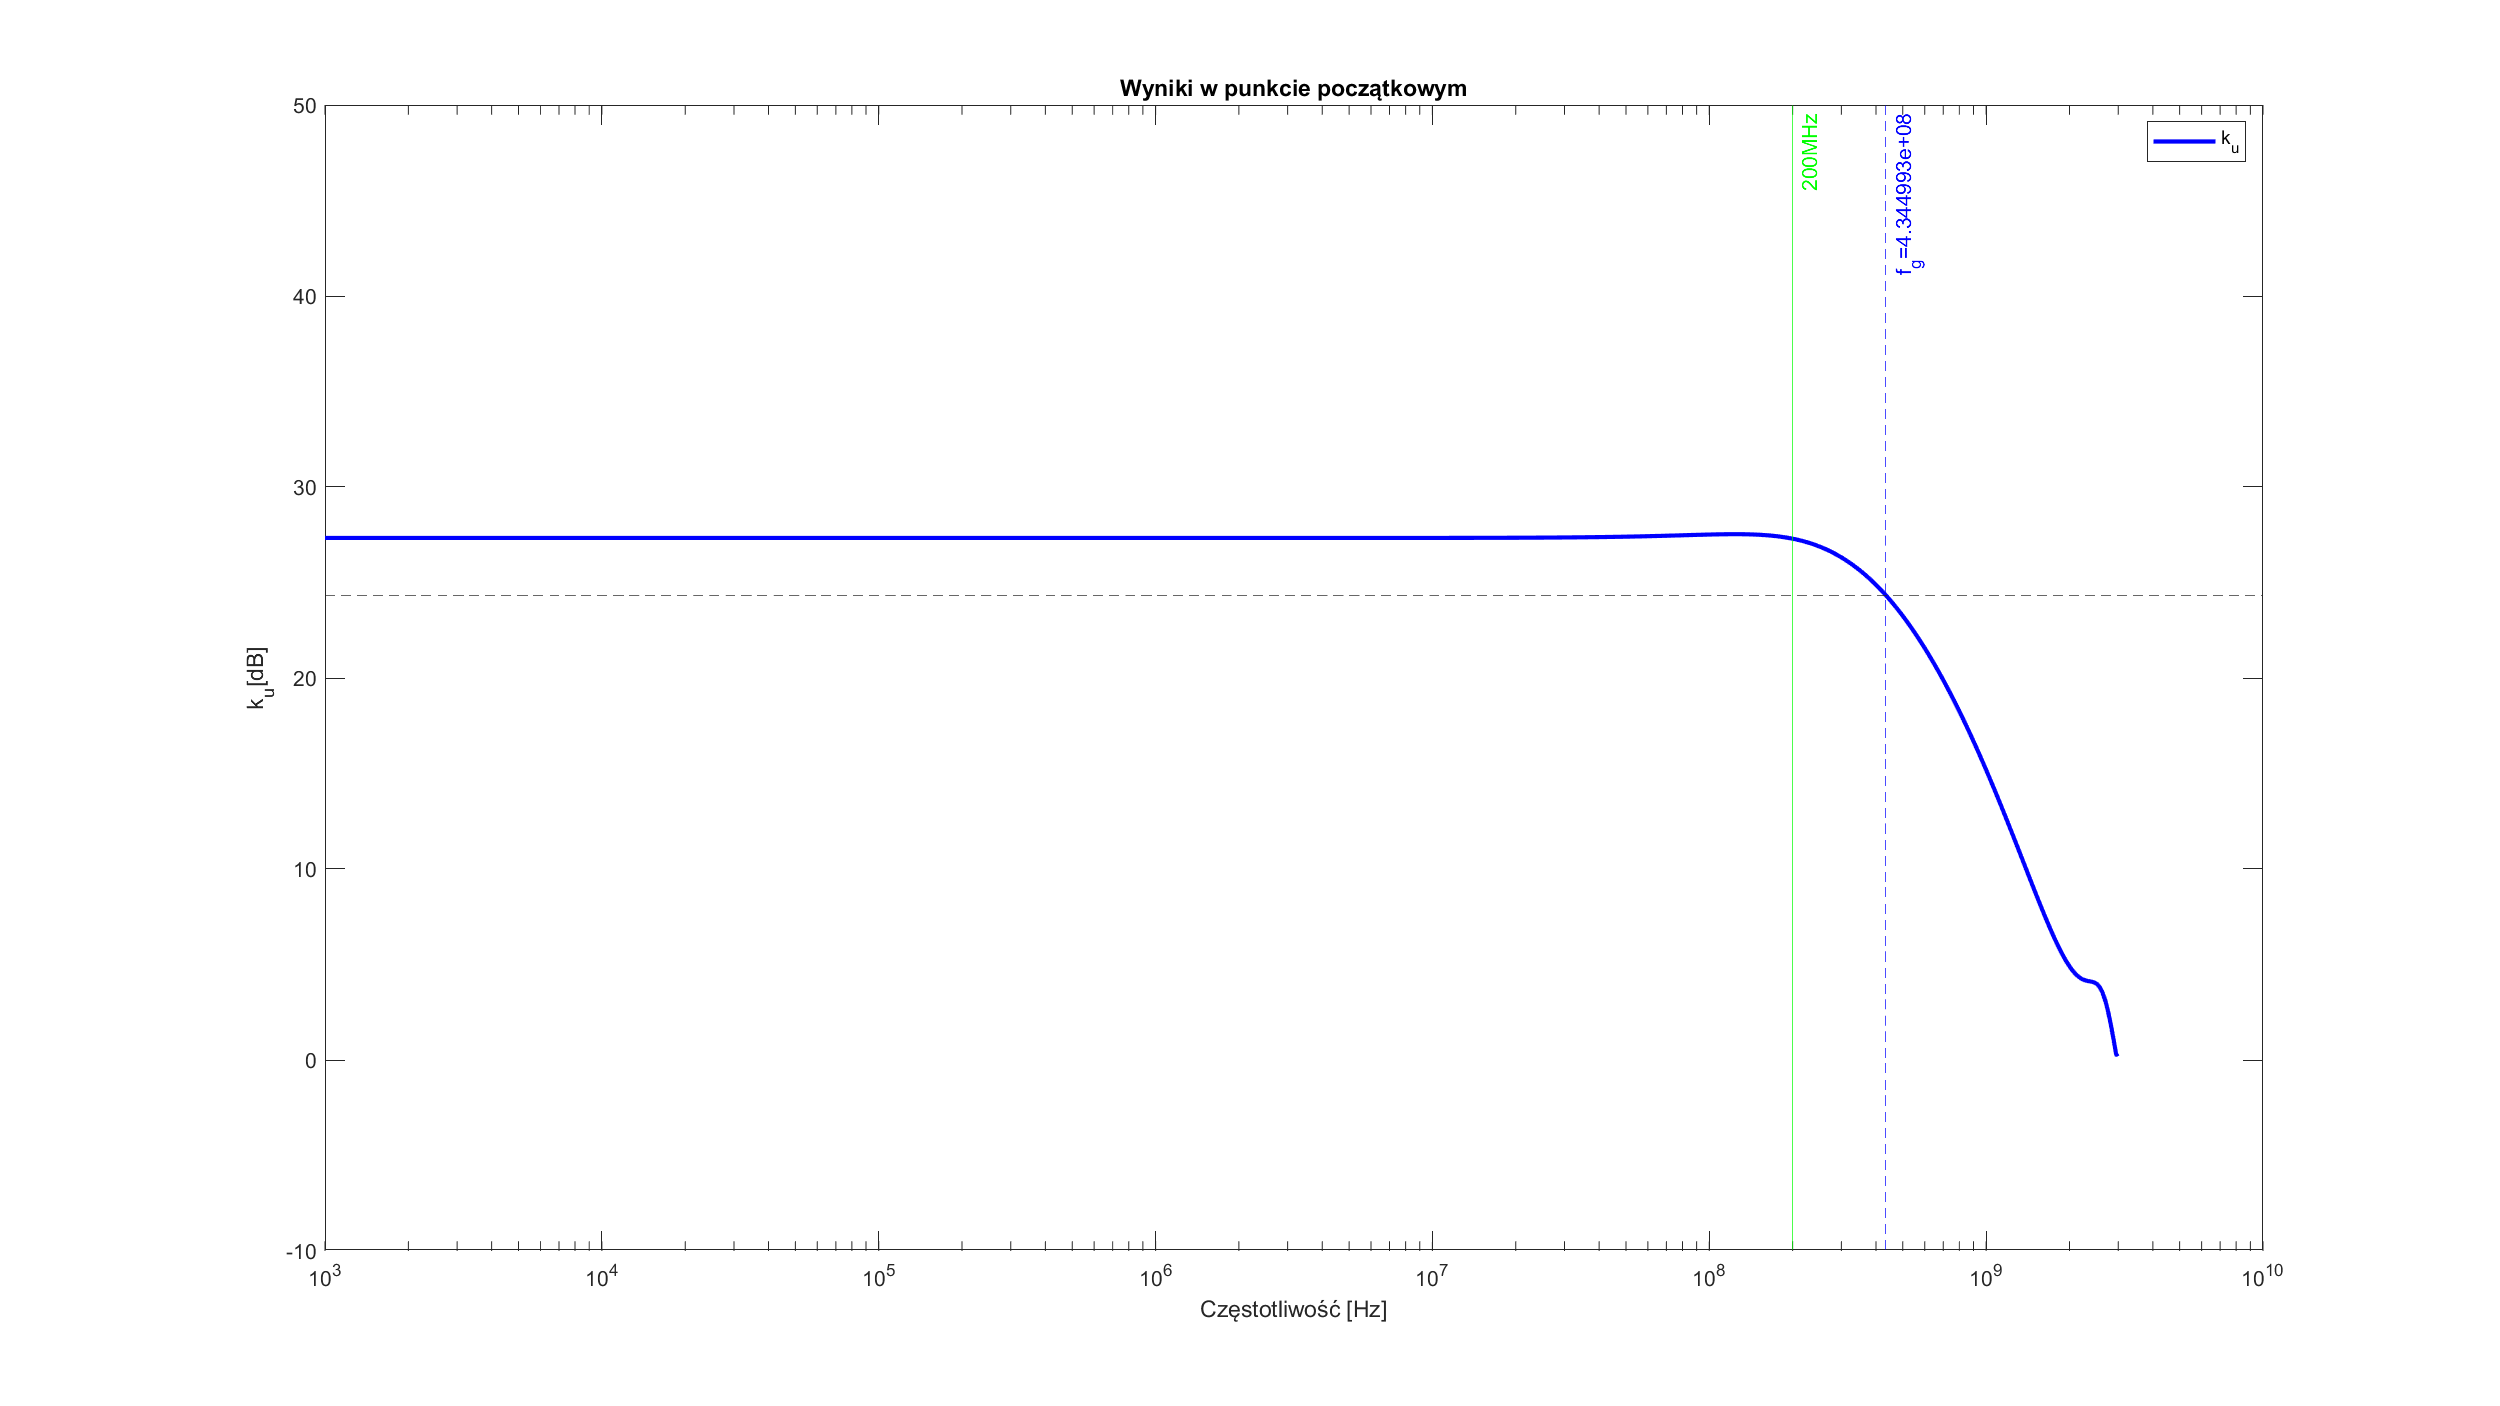
\includegraphics[width=12cm]{graphics/starting_point.png}
    \centering
    \caption{Charakterystyka układu w punkcie startowym.}
\end{figure}

Jak widać spełnione są warunki postawione w zadaniu (minimalna wartość wzmocnienia to 20 dB, przy źródle AC mającym 1 V amplitudy) oraz wzmacniacz pracuje prawidłowo (symulacja czasowa wykonana w LTSpice potwierdziła prawidłową pracę układu).
\pagebreak

Aby potwierdzić, że Matlab i Spice zwracają te same wyniki przeprowadzono symulację w LTSpice:
\begin{figure}[h]
    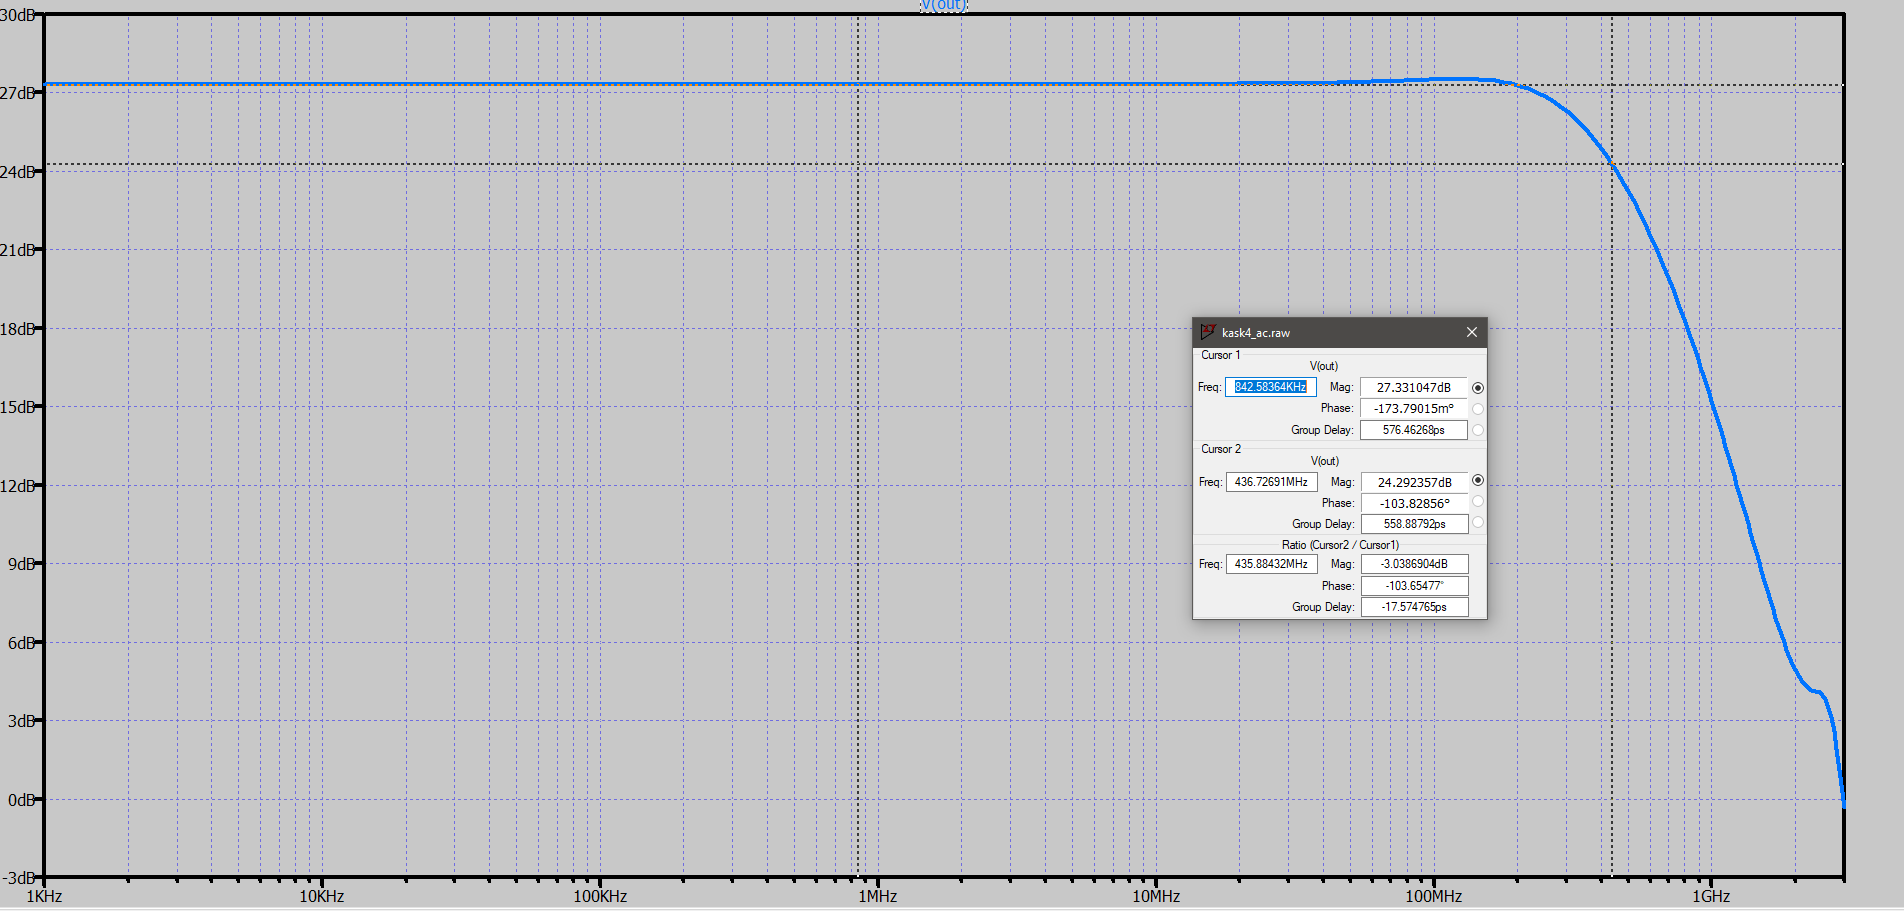
\includegraphics[width=12cm]{graphics/starting_point_spice.png}
    \centering
    \caption{Charakterystyka układu w punkcie startowym.}
\end{figure}



\section{Wyznaczanie parametrów roboczych, gładkość funkcji celu, opis kodu}
\subsection{Wyznaczanie parametrów roboczych}
W zadaniu badane są trzy parametry: częstotliwość graniczna, wzmocnienie oraz podbicie charakterystyki.

\subsubsection*{Podbicie $b$}
Podbicie rozumiane jest jako różnica między wzmocnieniem $k_{u0}$ a maksymalnym wzmocnieniem jakie osiąga charakterystyka ($b(\textbf{x})=max(k_{u}(\textbf{x}))-b_{max}$).
Maksimum charakterystyki jest wyznaczane przez interpolację (wielomian drugiego stopnia). Pozwala to dokładniej ustalić maksymalne wzmocnienie i wygładza funkcję ograniczeń.
Efekty interpolacji widać na poniższym wykresie:
\begin{figure}[h]
    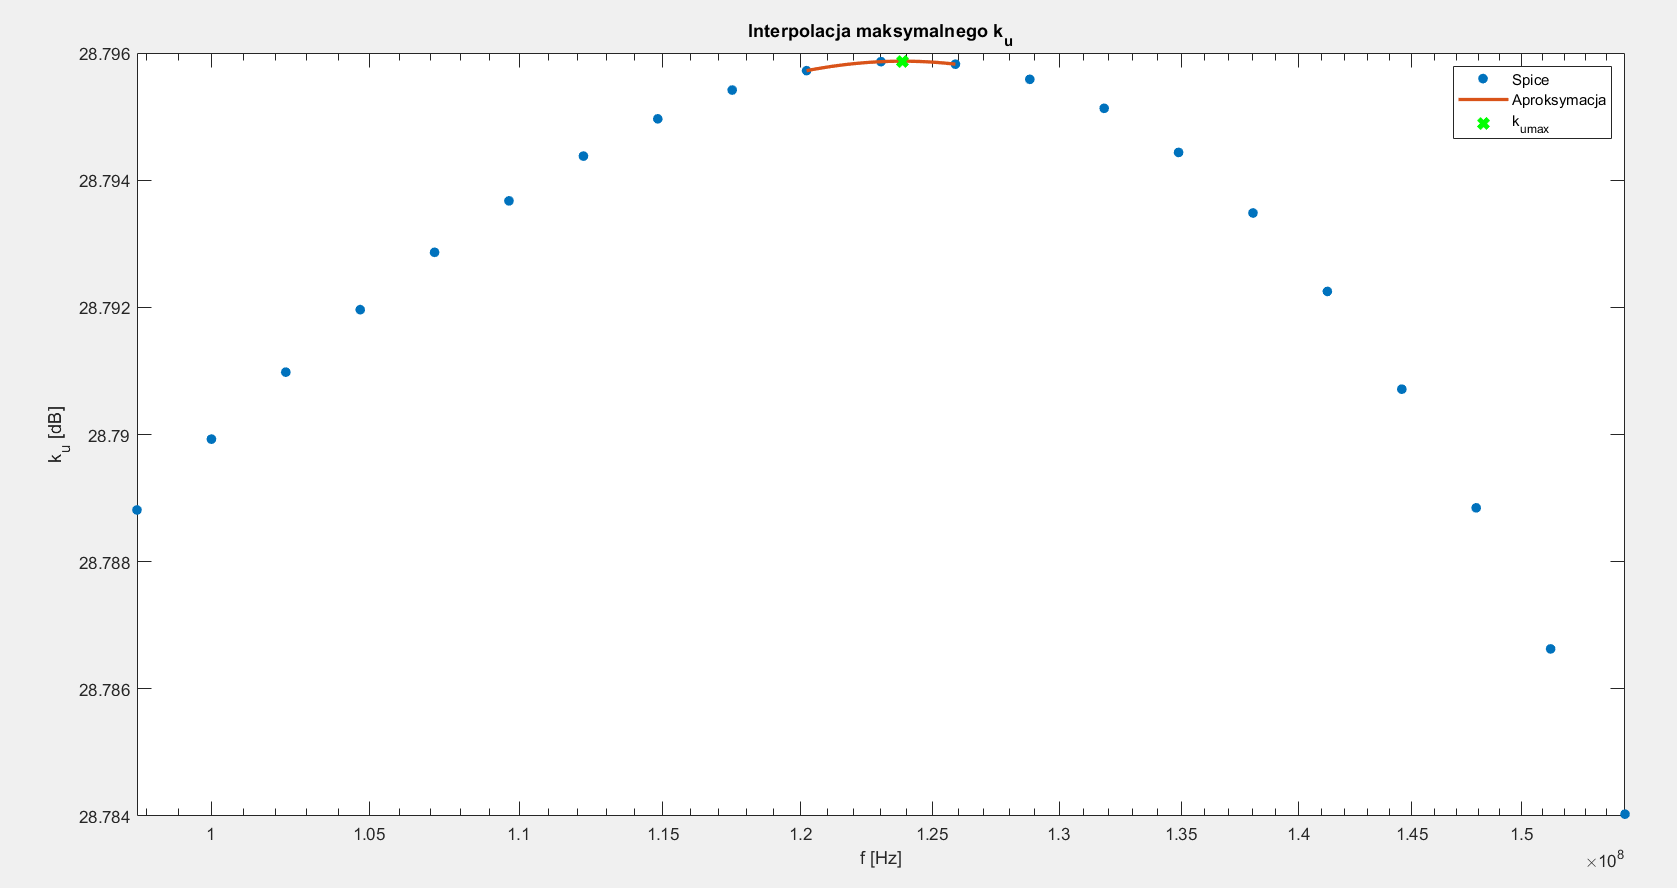
\includegraphics[width=8cm]{graphics/max_ku_interp.png}
    \centering
    \caption{Interpolacja maksimum charakterystyki.}
\end{figure}
\pagebreak
\subsubsection*{Wzmocnienie małoczęstotliwościowe $k_{u0}$}
Wzmocnienie $k_u$ rozumiane jest jako wartość wzmocnienia pozyskana z danych $U^{AC}_{out}(x,f)$ dla częstotliwości 1 KHz.

\subsubsection*{Częstotliwość graniczna $f_g$}
Częstotliwość graniczna wyznaczana jest jako częstotliwość, dla której wzmocnienie względem $k_{u{_0}}$ spada o 3 dB.
Ponieważ LTSpice zwraca wyniki w postaci punktów, uznano, że wymagana jest interpolacja częstotliwości granicznej. Interpolacja pozwoliła zminimalizować ''skoki'' w funkcji celu. Do interpolacji wykorzystano wielomian drugiego stopnia. Wynik interpolacji przedstawia poniższy wykres:
\begin{figure}[h]
    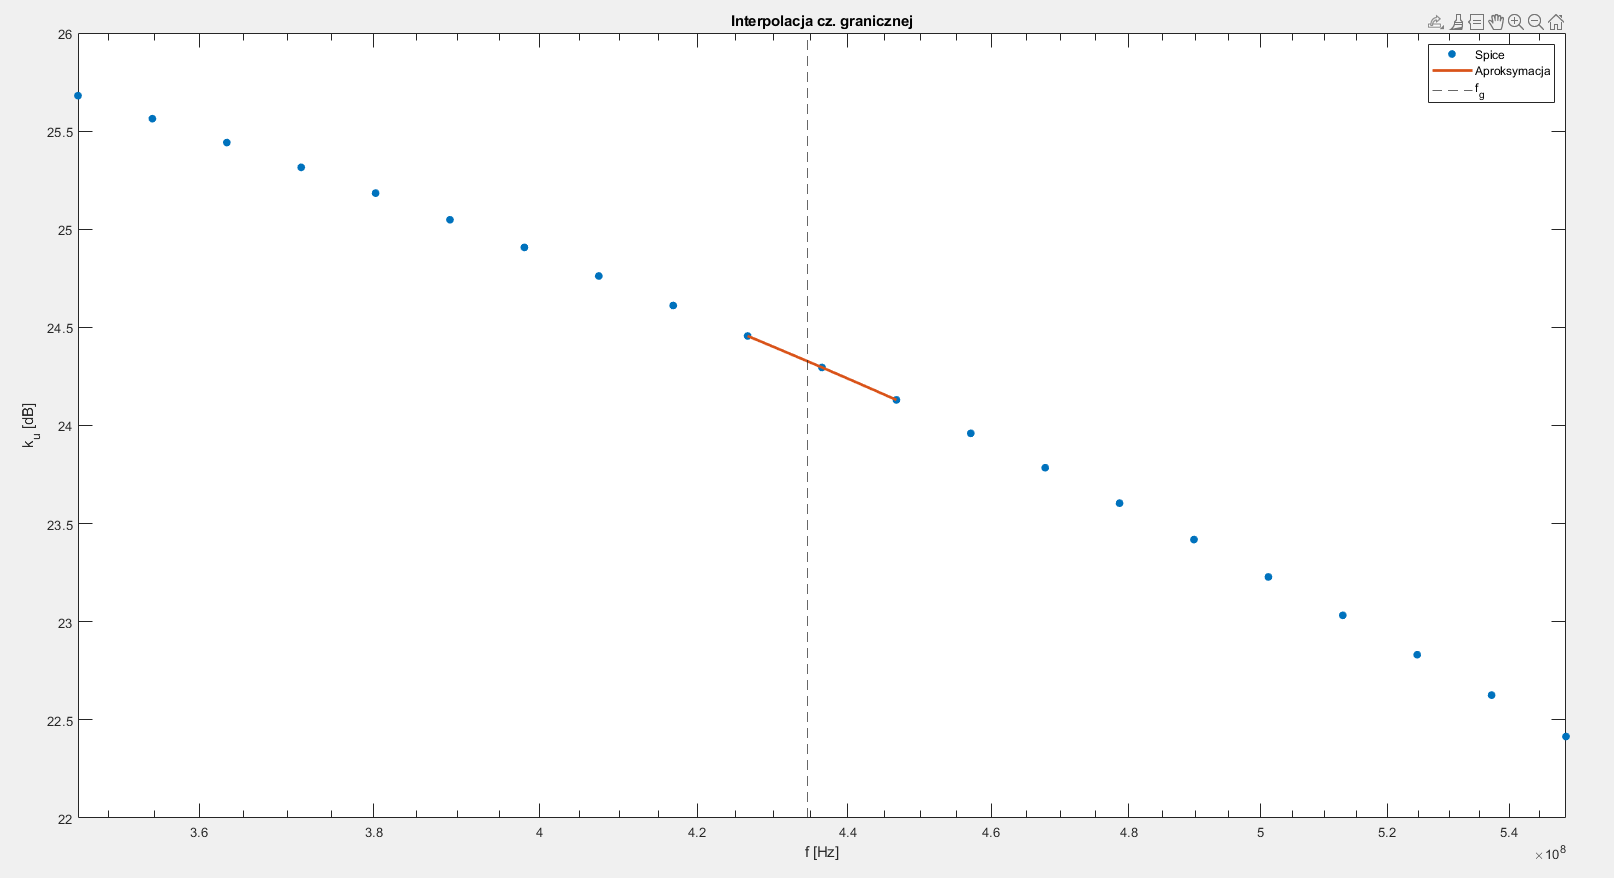
\includegraphics[width=8cm]{graphics/fg_interp.png}
    \centering
    \caption{Interpolacja częstotliwości granicznej.}
\end{figure}



\subsection{Gładkość funkcji celu i ograniczeń}
Przyjęto, że funkcja celu, w obrębie odpowiednich wartości elementów układu, jest ciągła. Tak długo, jak w układzie zmieniane są wartości pojemności i rezystancji i
nie powodują nieprawidłowej pracy układu zawsze możliwe będzie otrzymanie charakterystyki, która, nawet jeśli nie spełnia wymagań projektowych, daje ''sensowne'' wartości parametrów roboczych (bez dużych skoków
np. wzrost wzmocnienia do 10000 dB).

Funkcje ograniczeń i celu mogą być w niektórych przypadkach niegładkie. Może dojść do takiej sytuacji, gdy aktualny zestaw wartości elementów spowoduje powstanie charakterystyki,
dla której niektóre z parametrów roboczych nie są możliwe do obliczenia lub nie mają fizycznego sensu (np. płaska charakterystyka na poziomie 0 dB spowoduje, że nie istnieje częstotliwość graniczna rozumiana wg. zasad zdefiniowanych
na początku raportu, funkcja obliczająca zwraca wtedy wartość NaN), lub gdy któreś z ograniczeń zablokuje dany punkt (np. w obliczaniu podbicia wykorzystano operator max). 
Punkty przejścia między ""dobrą"" a ""złą"" charakterystyką są właściwie punktami, gdzie funkcja nie jest ciągła (a w niektórych przypadkach także niegładka). Solver fmincon nie spełnia ograniczeń dla każdej iteracji, przez co teoretycznie może zdarzyć się np. płaska charakterystyka,
dla której niektóre parametry nie mają sensu (np. brak spadku częstotliwości o 3 dB), jednak wg. dokumentacji, fmincon jest w stanie wrócić z takich punktów do poprawnej pracy. Przeprowadzone próby wykazały jednak, że problem ten zachodzi bardzo rzadko i ma niewielki wpływ na optymalizację.

W przypadku optymalizacji wielokryterialnej zdecydowano się wykorzystać solver paretosearch (wykorzystujący wewnętrznie algorytm patternsearch), niegładkość funkcji celu i ograniczeń nie ma tutaj więc dużego znaczenia (metoda bezgradientowa).
\subsection{Opis kodu}
Dołączony katalog z kodem podzielony został na odpowiednie katalogi dla wyników (results, gdzie zapisany jest workspace z Matlaba i plots, wykresy) i plików dla symulacji(spice).
W katalogu głównym znajdują się skrypty i m-funkcje. W celu weryfikacji poprawności działania kodu można uruchomić skrypt starting\_point.m, który przedstawia wyniki w pkt. początkowym.

Aby uruchomić optymalizację należy uruchomić skrypt main.m. Po optymalizacji wyniki zostaną zapisane do odpowiednich folderów.

Aby nie czekać aż optymalizator zakończy pracę (ok. 5 minut) można wczytać gotowe wyniki za pomocą komendy load(""'results/latest.mat'"").

\subsubsection*{Opis plików}
\begin{itemize}
    \item main.m - główny skrypt realizujący zadanie optymalizacji.
    \item display\_results.m - Skrypt wyświetlający wyniki optymalizacji. Uruchamiany automatycznie po main.m
    \item starting\_point.m - Skrypt obliczający wyniki w pkt. startowym. Do weryfikacji działania funkcji.
    \item optmization\_wrapper.m - funkcja będąca ""nakładką"" na optymalizator pozwalającą na współdzielenie między optymalizatorem a funkcjami celu i ograniczeń
          obliczonych wartości. Funkcja ta wykorzystuje zagnieżdżone funkcje celu i ograniczeń (oraz skalowania). Wszystkie ustawienia (dolne i górne ograniczenia, opcje itp.) znajdują się w tym pliku.
    \item multiobj\_optimization\_wrapper.m - Funkcja będąca ""nakładką"" na optymalizator wielokryterialny. Podobnie jak w wersji jednokryterialnej steruje całym procesem optymalizacji.
    \item get\_fg.m - Funkcja obliczająca częstotliwość graniczną.
    \item boost.m - Funkcja obliczająca podbicie charakterystyki.
    \item extract\_results.m - Funkcja odczytująca dane z pliku output\_results powstającego przez funckję output\_fun.
    \item modify\_params.m - Funkcja modyfikująca parametry w pliku params.inc
    \item output\_fun.m - Funkcja wyjściowa dla optymalizatora.
    \item run\_sim.m - Funkcja uruchamiająca symulator LTSpice.
    \item get\_working\_params.m - Funkcja obliczająca podbicie, częstotliwośś graniczną i wzmocnienie.
    \item LTspice2Matlab.m - Funkcja do odczytu danych z LTSpice.
\end{itemize}

\section{Propozycja rozwiązania numerycznego}
\subsection{Algorytm, skalowanie}
\subsection*{Solver i algorytm optymalizacji jednokryterialnej}
Jako solver wykorzystano fmincon z domyślnym algorytmem (Interior Point). Zdecydowano się na wykorzystanie
metod gradientowych, ponieważ założono gładkość funkcji dla danych ograniczeń. Po przeprowadzonych próbach optymalizacji uznano, że założenie jest słuszne (nieciągłości jedynie w punktach nie dających wyników o sensie fizycznym, widoczna poprawa parametrów układu, wyraźna zbieżność).
Wpływ niegładkości wprowadzanej przez ograniczenie podbicia nie spowodował ani razu przerwania optymalizacji.

Po próbach przeprowadzonych w LTSpice ustalono, że niektóre elementy mają większy wpływ na układ niż inne, jednak, przy różnych kombinacjach wartości, wpływ rożnych elementów jest trudny do przewidzenia.
Stwierdzono np. że zmniejszanie wartości REE1 powoduje wzrost wzmocnienia przy spadku pasma, manipulowanie pojemnością CEE wpływa na pasmo, CG na podbicia itp.
Ponieważ nie znaleziono jednoznacznej zależności (działanie na kształt algorytmu Gaussa-Seidla) postanowiono nie ograniczać liczby optymalizowanych zmiennych, a jedynie zadbać o odpowiednie
ograniczenia kostkowe parametrów.
\subsection*{Solver i algorytm dla optymalizacji wielokryterialnej}
W praktyce ciężko określić co jest ""dobrym"" rozwiązaniem zadania wielokryterialnego. Przeważnie mamy do czynienia z optymalizowaniem parametrów gdzie poprawa jednego powoduje pogorszenie pozostałych.
Aby znaleźć rozwiązanie zadanego problemu zdecydowano się użyć solvera paretosearch (wykorzystującego algorytm patternsearch) do wyznaczenia zbioru Pareto, który powinien dać wybór w kwestii czy bardziej interesuje użytkownika
wzmocnienie czy pasmo.

Ponieważ patternsearch jest algorytmem bezgradientowym ewentualny brak gładkości f. celu i ograniczeń nie ma tutaj dużego znaczenia.
\subsection*{Skalowanie}
Zarówno wektor wartości elementów jak i funkcja celu zostały przeskalowane.

W przypadku wektora parametrów optymalizowanych zastosowano proste skalowanie do 1 względem punktu startowego $\frac{x}{x_0}$.
W badanym przypadku wartości są podobnego rzędu (jednostki zostają dopisane dopiero w funkcji modyfikującej plik z parametrami), jednak dla przejrzystości postanowiono wykonać
skalowanie wektora względem wektora startowego.

W przypadku funkcji celu iloczyn wzmocnienia i częstotliwości granicznej sięga rzędu $10^9$.
Aby usprawnić pracę optymalizatora wyjście z zaimplementowanej funkcji celu jest postaci $-log_{10}(GBW)$.

W przypadku optymalizacji wielokryterialnej częstotliwość graniczna zwracana jest w postaci $-log_{10}(f_g)$.

Wartości wzmocnienia nie przekraczają zakresu od kilku do kilkuset decybeli. Uznano, że nie jest tu konieczne skalowanie. 

\pagebreak
\begin{center}
    \title{ \huge \textbf{Etap 2}}
    \addcontentsline{toc}{section}{Etap 2}

\end{center}

\section{Optymalizacja}
\subsection{Ocena poprawności założeń}
Biorąc pod uwagę wyniki optymalizacji zarówno jedno jak i wielokryterialnej uznano, że założenia z etapu 1 były prawidłowe.

W przypadku optymalizacji jednokryterialnej zauważono poprawę o ok. 68\% ($\frac{GBW_{opt}}{GBW_{0}}=1.678$) względem punktu startowego. Wszystkie ograniczenia zostały także spełnione, a optymalizator
zwraca flagę o możliwości istnienia minimum lokalnego. Omawiane wcześniej założenia dotyczące sytuacji, gdy funkcja celu lub ograniczeń zwróci wartość NaN także okazały się słuszne i optymalizator jest w stanie wrócić do poprawnej pracy z takich punktów.

W przypadku optymalizacji wielokryterialnej wnioski są podobne.

Optymalizator wyznacza granicę Pareto, która układa się w ""sensowny"" kształt. Dodatkowo widać, że punkt startowy jest punktem zdominowanym, natomiast te wyznaczone prze algorytm są pareto-optymalne.
Punkt wyznaczony jako optymalny w optymalizacji jednokryterialnej także leży na wyznaczonej granicy Pareto.

Mimo, że punktem wyjścia z optymalizatora jest przekroczenie czasu (30 min) uznano, że (badając kształt i wartości na granicy Pareto),
że optymalizacja przebiegła poprawnie. Wszystkie ograniczenia także są spełnione.

\subsubsection{Funkcje celu i ograniczeń, skalowanie, dokładność i gładkość}
W etapie 2 nie wprowadzono zmian dotyczących funkcji celu, ograniczeń, nie zmieniano także skalowania.
Założenia dotyczące gładkości funkcji także okazały się słuszne.

Optymalizacja GBW kończy się informacją ''Local minimum possible'', co oznacza, ze teoretycznie istnieje lepszy punkt niż wynikowy, jednak przyyrsoty dla wartości funkcji celu są mniejsze od
ustawionego kroku dla solvera. Teoretycznie można by uruchomić optymalizator z tego punktu jeszcze raz, z mniejszym krokiem, jednak biorąc pod uwagę ograniczenie ze strony wzmocnienia układu (rysunek) uznano,
że wyliczony punkt jest wystarczająco bliski optymalnego.

\subsubsection{Wybrane algorytmy optymalizacji}
Na podstawie wyników oraz przebiegu optymalizacji uznano, że dobór algorytmów był prawidłowy.

W przypadku optymalizacji jednokryterialnej algorytmem był domyślny algorytm gradientowy Interior-Point.
Zadanie udało się rozwiązać poprawnie oraz optymalizator zakończył pracę z informacją o możliwości istnienia lokalnego minimum. Jako że
powyższy wybór jest wyborem z etapu 1 uznano, że wybór był słuszny i nie zmieniano algorytmu.

W przypadku optymalizacji wielokryterialnej wykorzystano sugerowany w etapie 1 algorytm patternsearch. Biorąc pod uwagę punkty na wyznaczonej granicy Pareto także uznano, ze wybór jest słuszny.
\subsubsection{Wykorzystane opcje dla algorytmów}
W przypadku solvera dla optymalizacji jednokryterialnej zmieniono następujące opcje:
\begin{itemize}
    \item ''FinDiffRelStep''=1e-2 - zmieniono domyślną długość kroku, gdyż dla niektórych punktów domyślny krok powodował zbyt małe przyrosty funkcji celu.
    \item ''OutputFcn'',@output\_fun - zaimplementowano własną funkcję wyjściową. Dokładny opis w etapie 1 oraz w kodzie matlaba.
\end{itemize}

W przypadku optymalizacji wielokryterialnej:
\begin{itemize}
    \item 'ParetoSetSize' - ustalono maksymalny rozmiar zbioru Pareto. Optymalizator jest w stanie obliczyć dość dużo punktów, jednak zajmuje to bardzo dużo czasu. Uznano, że zbiór o wielkości 50 punktów na pewno pozwoli
          wywnioskować czy solver działa poprawnie i czy założenia były słuszne. W przypadku jednak, gdyby obliczenie 50 punktów trwało zbyt długo wproadzono także ograniczeń dot. maksymalnego czasu.
    \item 'InitialPoints' - Solver paretosearch można zainicjować punktami startowymi. W tym przypadku ""zaporponowano"" punkt startowy taki sam jak dla optymalizacji jednokryterialnej, gdyż spełniał on wszystkie ograniczenia.
    \item 'MaxTime' - Ograniczenia dotyczące czasu optymalizacji. Ustawiono na 1800 s, w tym czasie optymalizator wyznaczył ok. 35 punktów na granicy Pareto. Uznano, że zbiór ten dobrze pokazuje działanie optymalizatora oraz daje pogląd co do zachowania układu.
\end{itemize}

\pagebreak
\subsection{Podsumowanie przebiegu optymalizacji}
\subsubsection{Optymalizacja jednokryterialna}
\subsubsection*{Porównanie obiektu przed i po optymalizacji}
Wyniki optymalizacji jednokryterialnej zobaczyć można na poniższym wykresie:
\begin{figure}[h]
    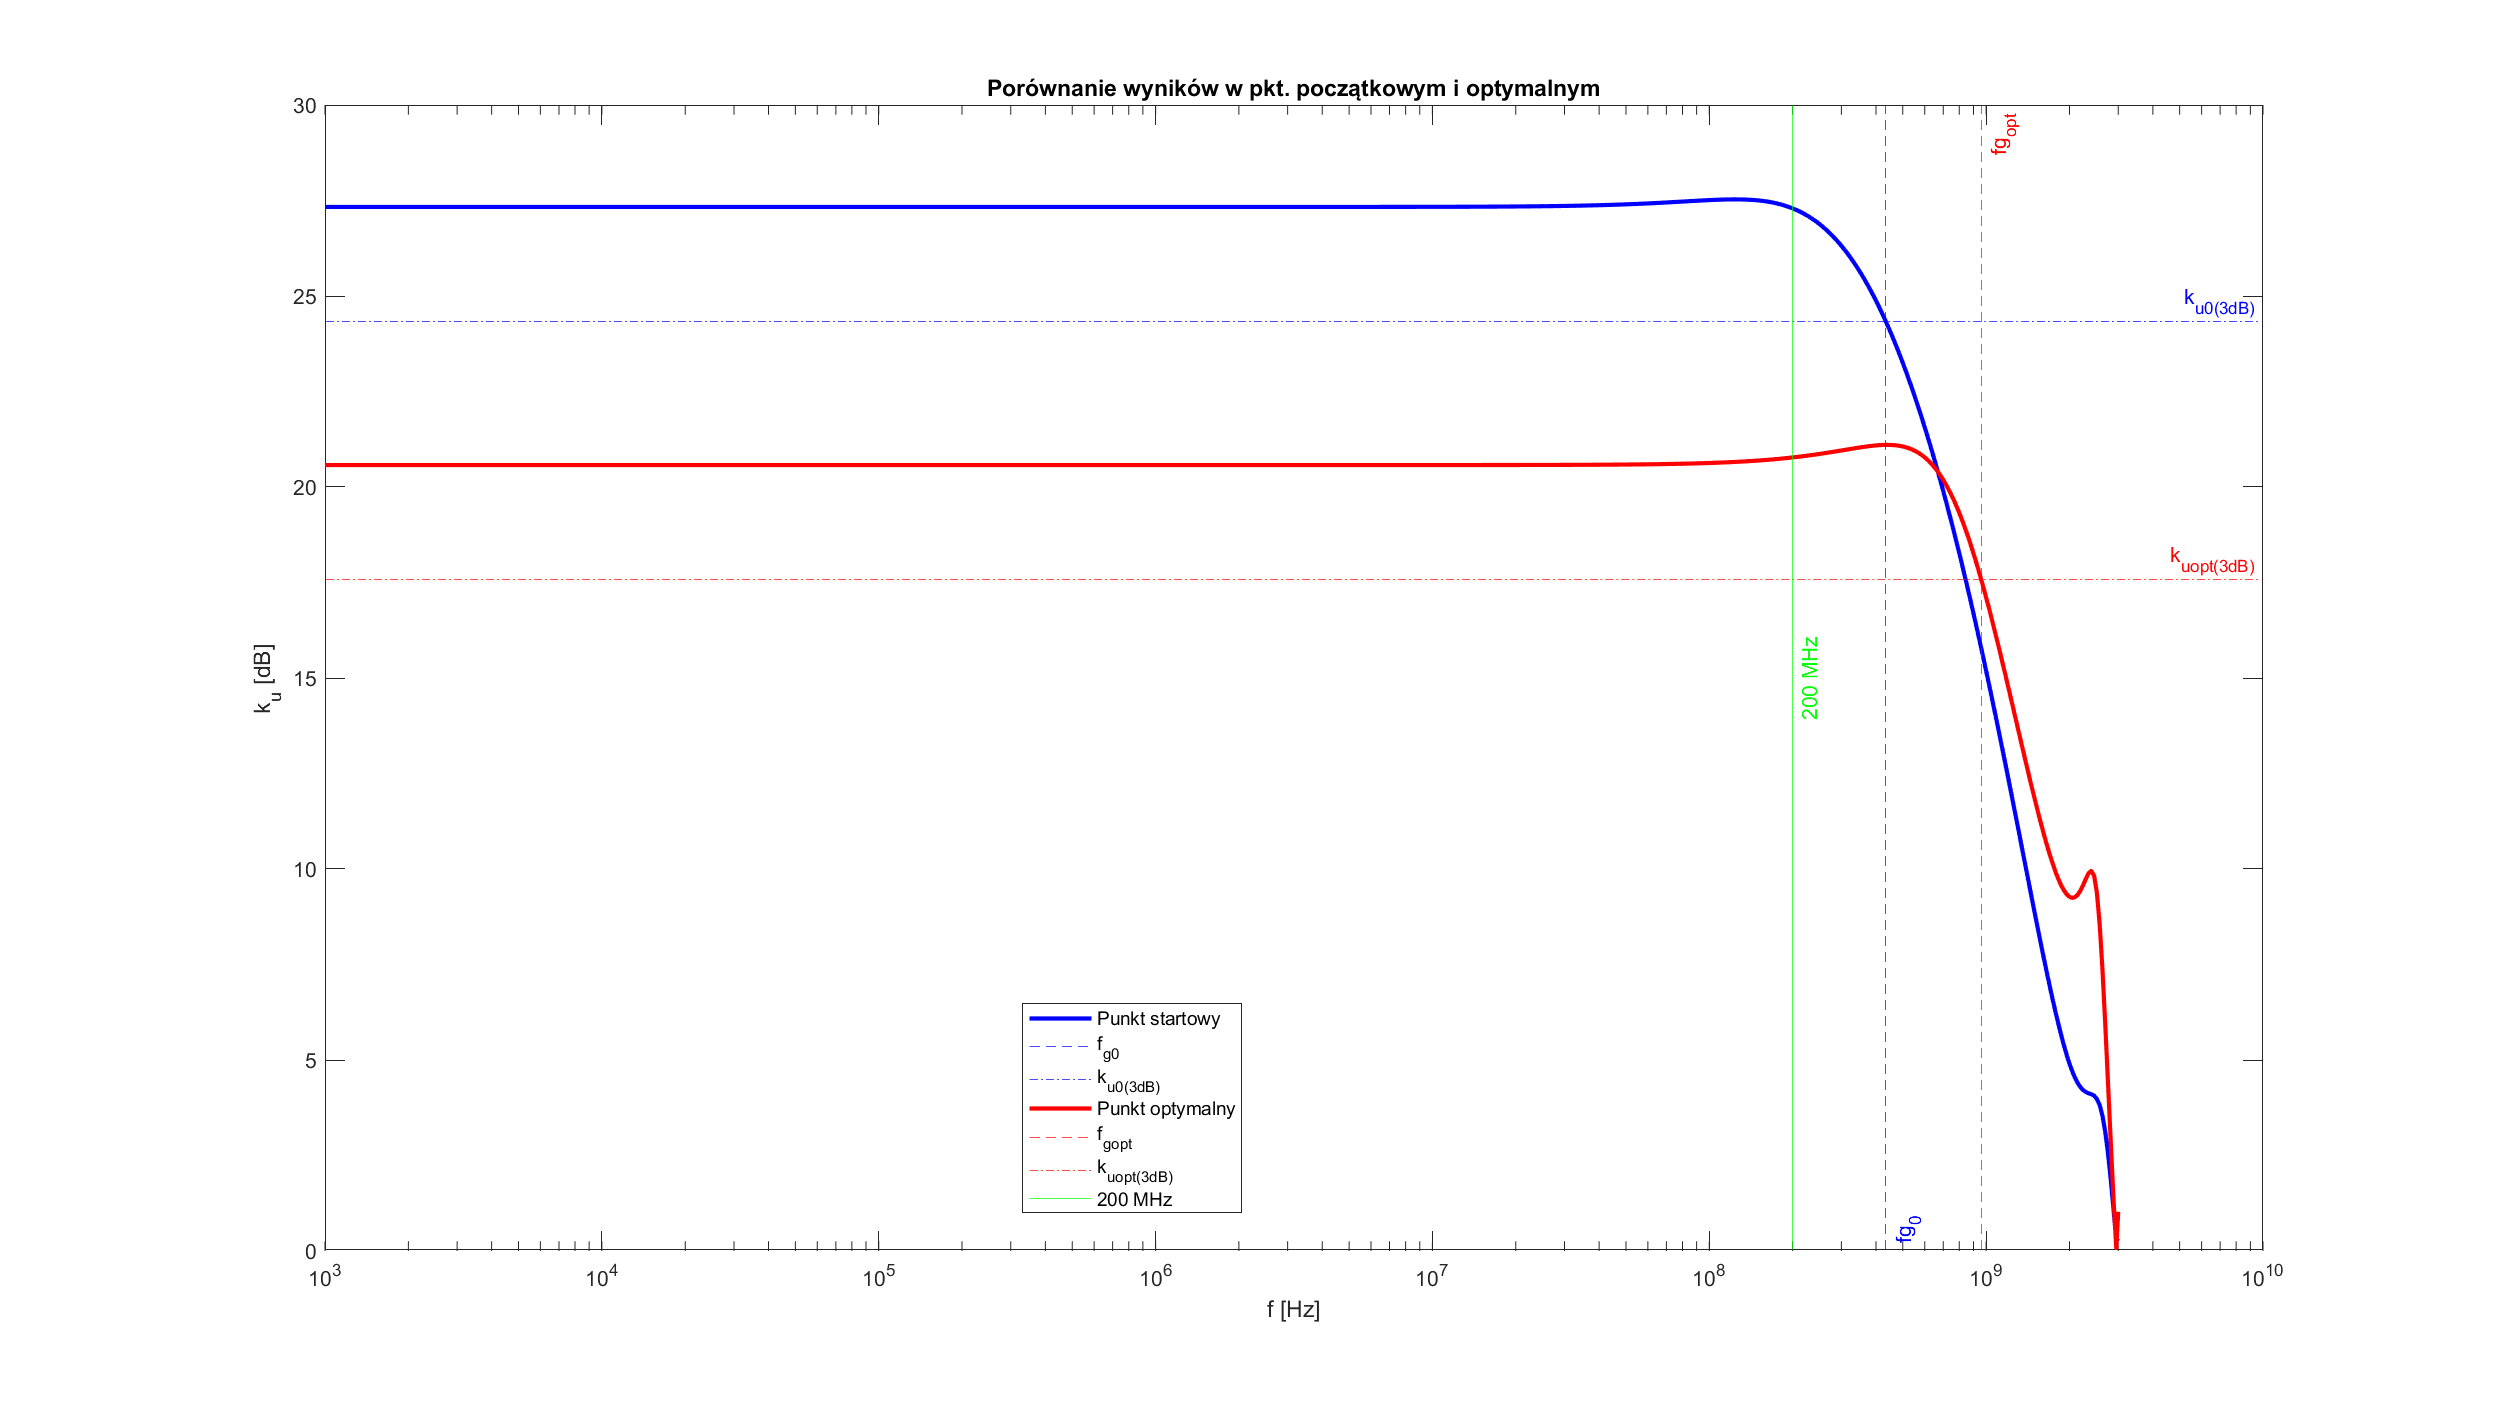
\includegraphics[width=12cm]{graphics/comparison.png}
    \centering
    \caption{Porównanie wyników w punkcie startowym i optymalnym.}
\end{figure}

W trakcie optymalizacji zauważono, że optymalizator zdecydowanie bardziej faworyzuje rozszerzanie pasma zamiast podniesienia wzmocnienia.
Prowadzi to do sytuacji, gdy wzmocnienie praktycznie osiąga wartość minimalną, natomiast zyskujemy duże pasmo.

Ograniczenie wzmocnienia jest więc ograniczeniem aktywnym (gdybyśmy pozwolili optymalizatorowi dalej zmniejszać wzmocnienie poszerzałby on dalej pasmo).

Jeżeli użytkownikowi zależy na dużym iloczynie GBW ale dla większego wzmocnienia można albo zwiększyć minimalne wzmocnienie lub nałożyć górne ograniczenie na pasmo (wtedy optymalizator
powinien starać się podbijać wzmocnienie). Jednak ponieważ wynik spełnia założenia projektowe postanowiono nie modyfikować procesu optymalizacji.

Warto wspomnieć tutaj także o ograniczeniu dotyczącym podbicia.

W trakcie optymalizacji wielokryterialnej obserwowano przebiegi generowane przez symulator. Zauważono, że wiele przebiegów osiągało wysoką wartość zarówno wzmocnienia jak i pasma
jednak podbicie eliminowało takie punkty ze zbioru rozwiązań. Gdyby zwiększyć dopuszczalne podbicie być może uzyskano by lepszy punkt niż optymalny (z optymalizacji wielokryterialnej). To ograniczenie
także uznano za aktywne.
\subsubsection*{Wartości liczbowe funkcji celu i ograniczeń}
Informacje o przebiegu optymalizacji (ze zmiennej ```optim\_out```):
\begin{itemize}
    \item \textbf{Liczba iteracji:} 45
    \item \textbf{Liczba wywołań funkcji:} 478
    \item \textbf{Naruszenie ograniczeń:} 0
    \item \textbf{Wartość funkcji celu w p. optymalnym:} $f(\textbf{xopt})=1.9926\cdot 10^{10}$
    \item \textbf{Wartość parametrów w p. optymalnym:} \\ $ x_{opt}= \begin{bmatrix}     9.947 \Omega & 1.576 \Omega & 536.0 \Omega & 254.7 \Omega & 157.4 \Omega & 19.93 p & 125.7 p       \end{bmatrix}  $
    \item \textbf{Powód zakończenia:} ''Local minimum possible''
\end{itemize}

Dodatkowo nałożono ograniczenia kostkowe na optymalizowane wartości. Ograniczenia te zostały dobrane empirycznie po kilku próbach ręcznej optymalizacji układu.
Pozwalają one na maksymalnie 10 krotne zmniejszenie zmiennych ($ lb= \begin{bmatrix} 0.1 & 0.1& 0.1 & 0.1  & 0.1 & 0.1  \end{bmatrix} $), od góry zmienne ogarniczone się weflug wektora: $ ub= \begin{bmatrix} 2 & 2 & 5 & 5  & 10 & 10  \end{bmatrix} $
\pagebreak
Przebieg wartości funkcji celu zobaczyć można na poniższej grafice:
\begin{figure}[h]
    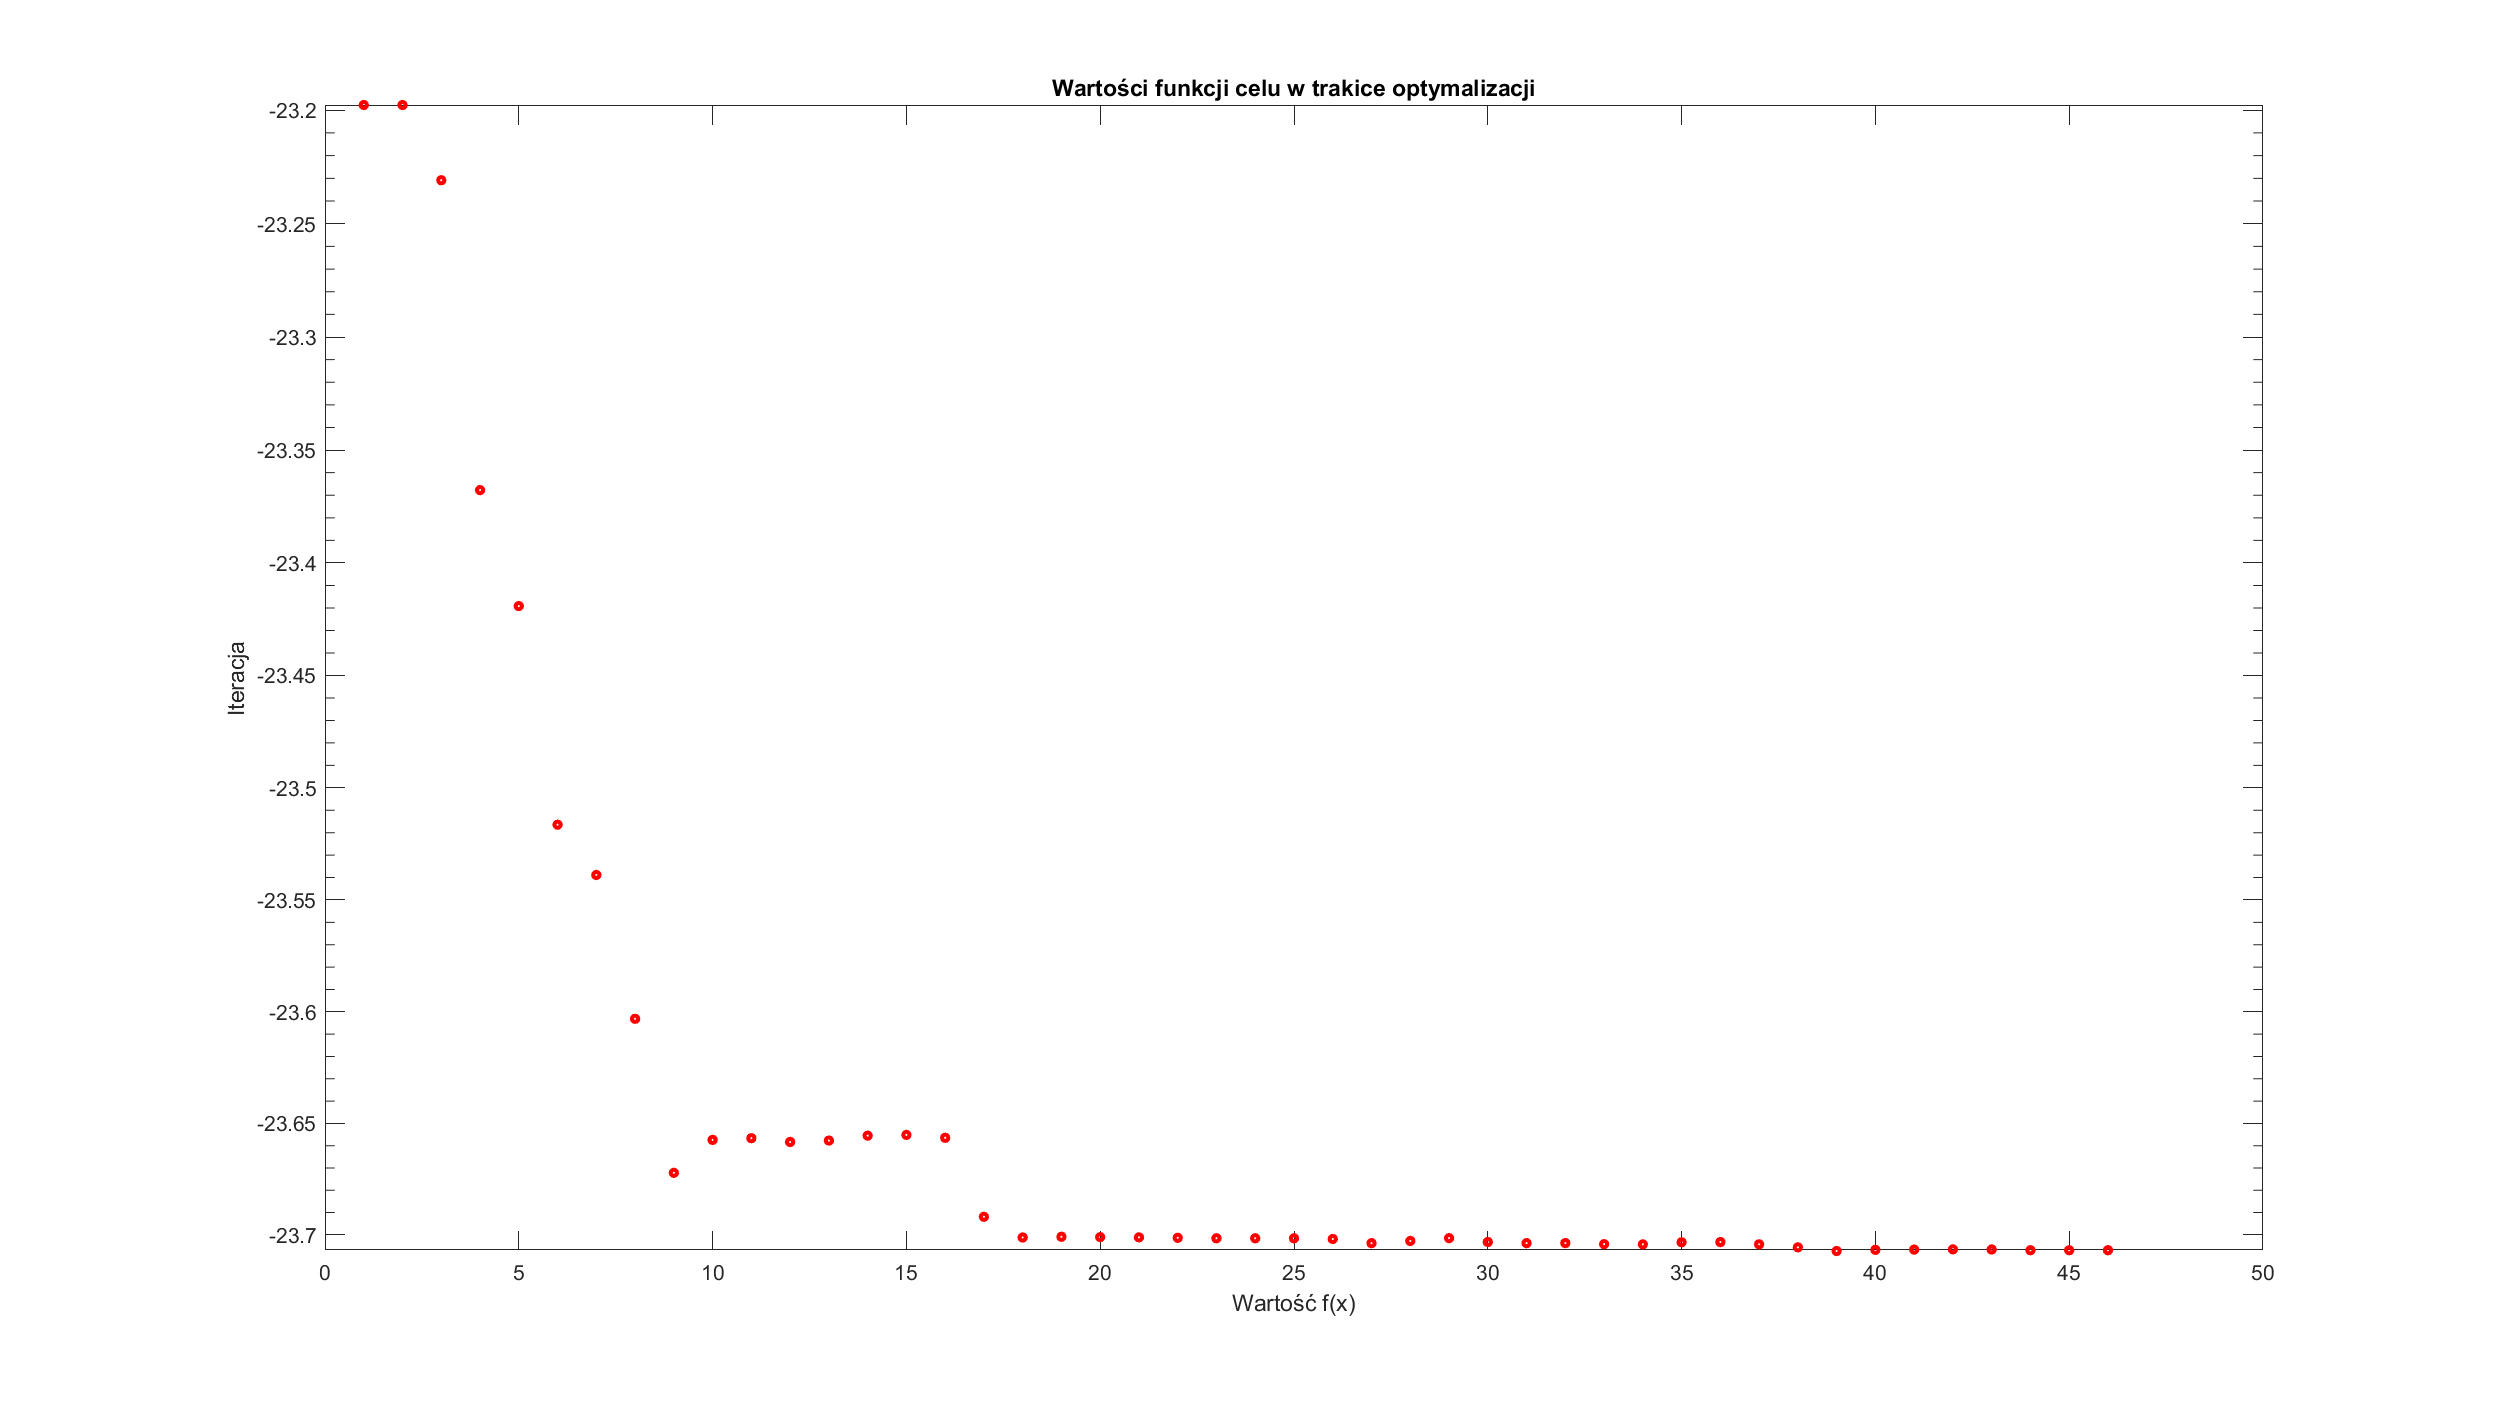
\includegraphics[width=12cm]{graphics/fval.png}
    \centering
    \caption{Przebieg wartości funkcji celu w trakcie optymalizacji.}
\end{figure}
Funkcja celu zbiega w sposób kwadratowy.

\begin{itemize}
    \item \textbf{Czy wskutek użycia optymalizacji zrealizowano wymagania projektowe?}\\
          Tak, wyniki mieszczą się w zadanych ograniczeniach projektowych.
    \item \textbf{Czy uzyskano widoczną poprawę własności obiektu?}\\
          Tak, GBW wzrosło o ok 68\% względem punkt początkowego. Uznano to za bardzo dobry wynik.
\end{itemize}
\subsubsection{Optymalizacja wielokryterialna}

\subsubsection*{Porównanie obiektu przed i po optymalizacji}
Wyniki optymalizacji wielokryterialnej przedstawiono jako zbiór Pareto:
\begin{figure}[h]
    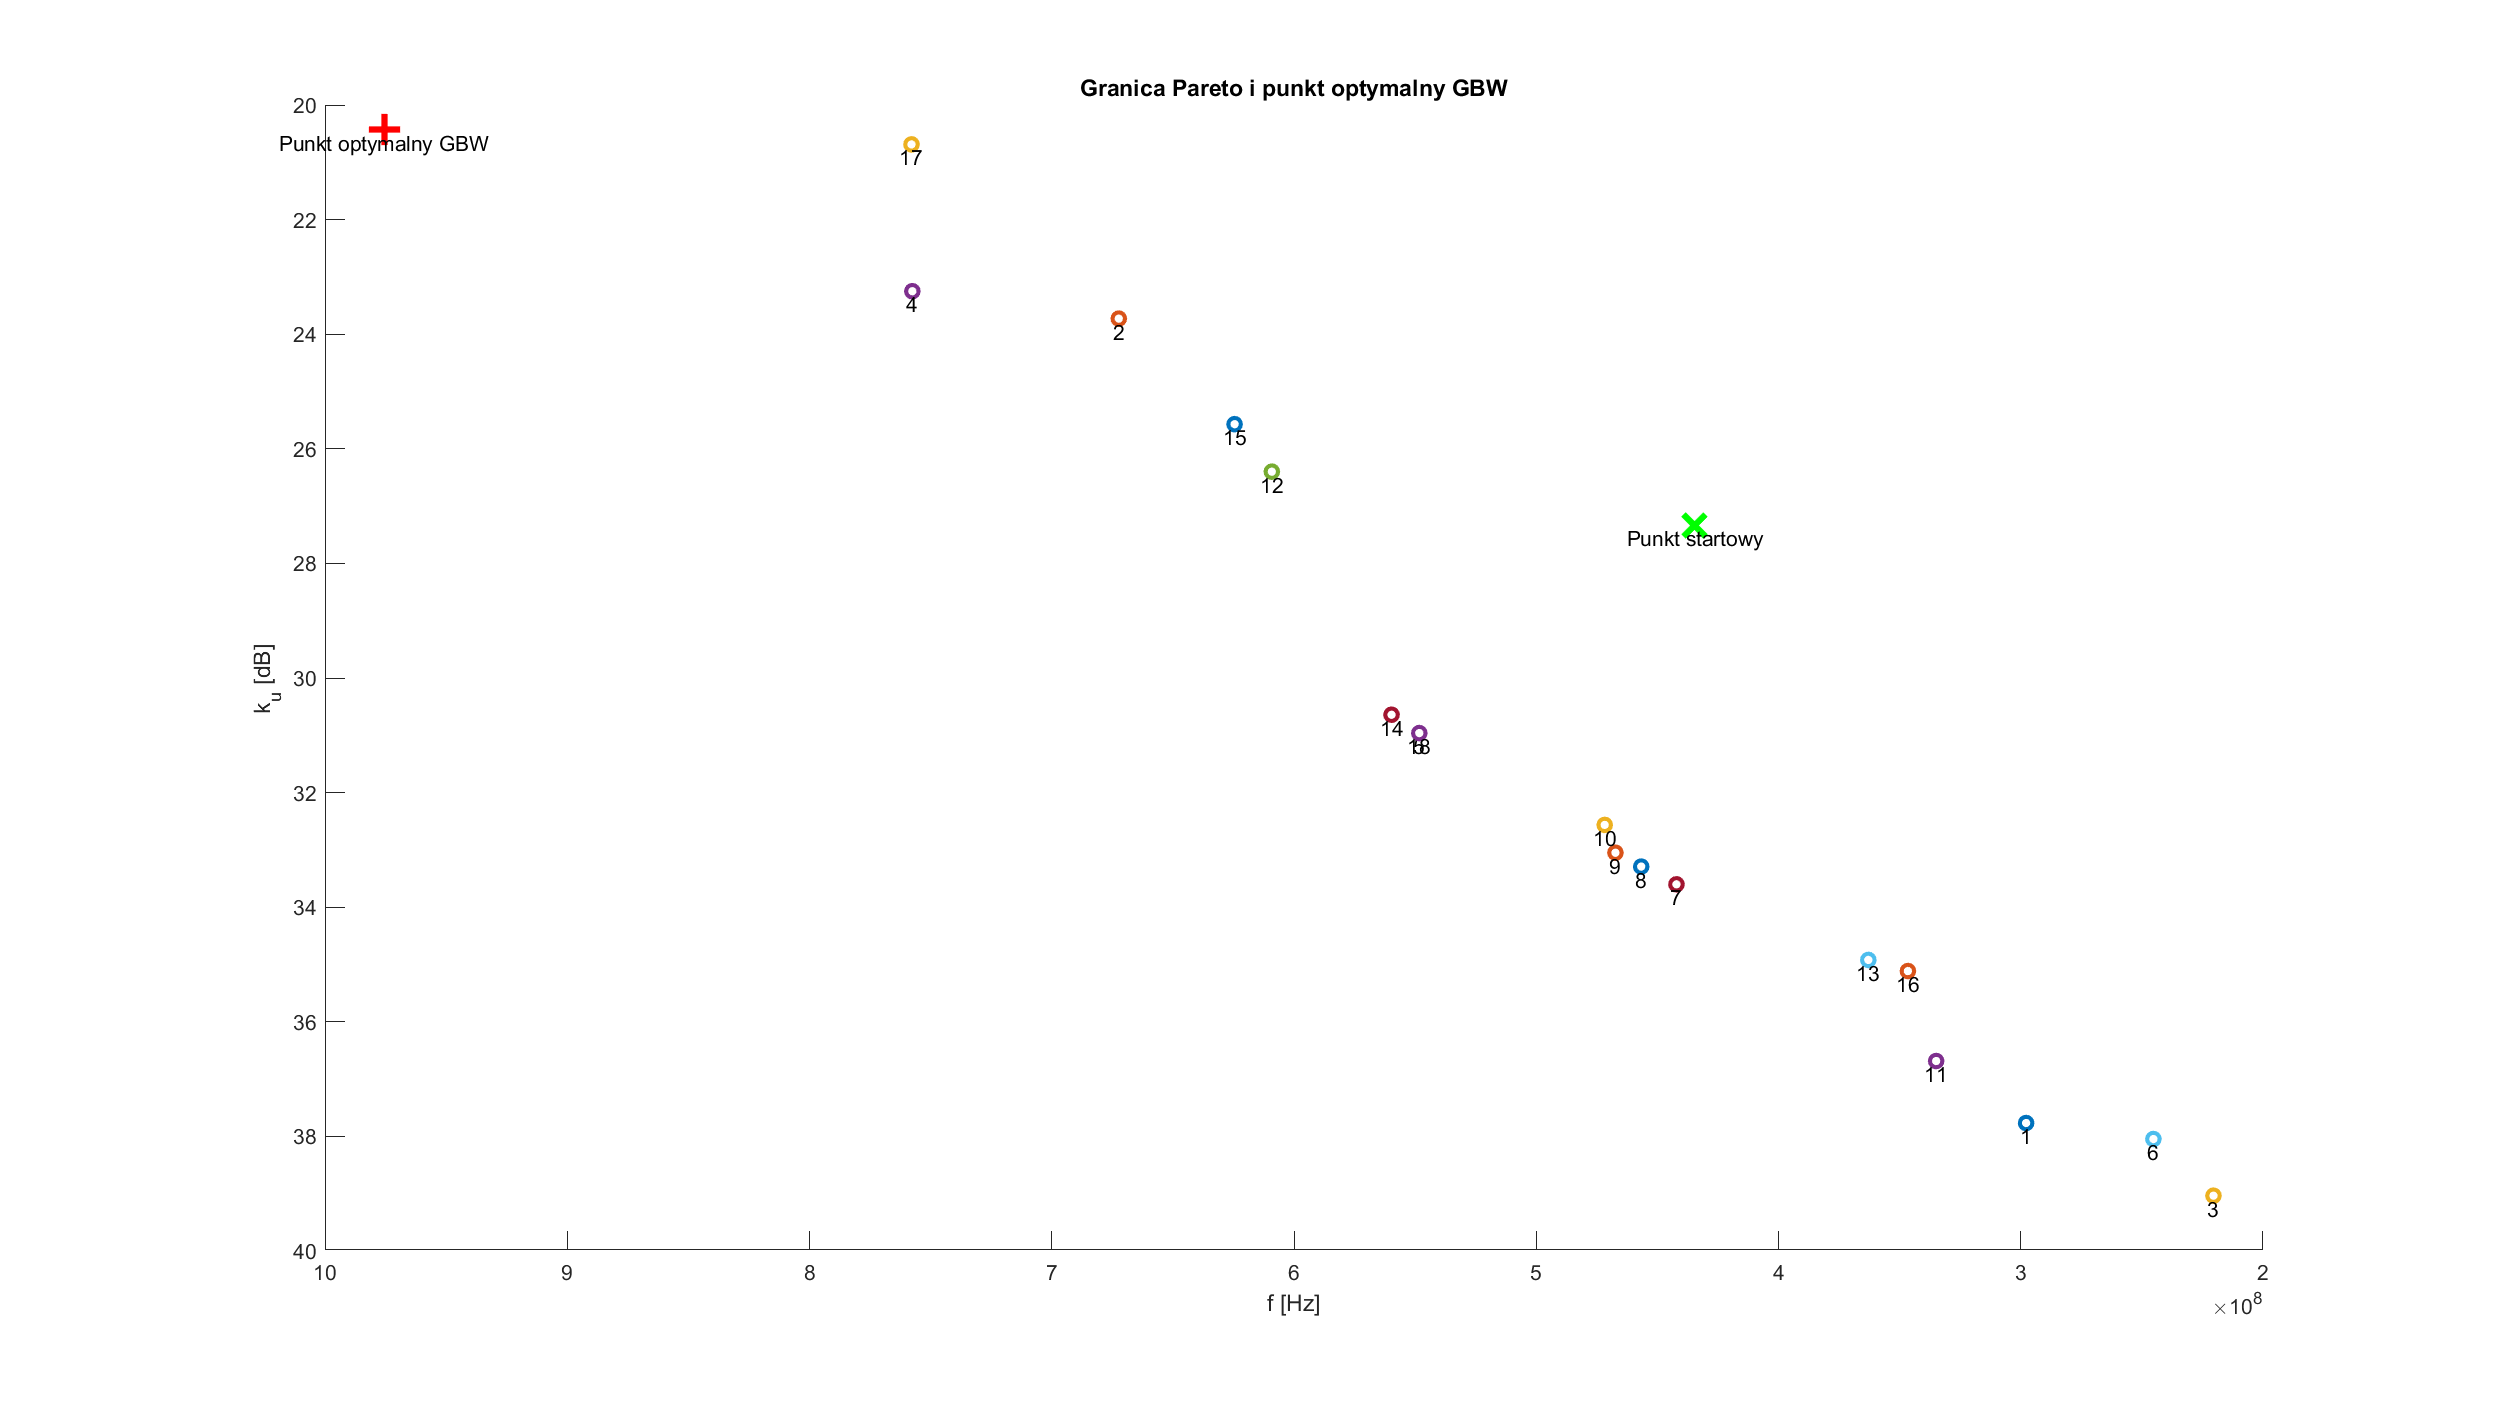
\includegraphics[width=12cm]{graphics/pareto.png}
    \centering
    \caption{Zbiór Pareto dla optymalizacji wielokryterialnej.}
\end{figure}

Jak widać każdy z obliczonych punktów jest lepszy zarówno w paśmie jak i wzmocnieniu od punktu startowego. Optymalizator spełnił więc swoje zadanie.
\subsubsection*{Wartości liczbowe funkcji celu i ograniczeń}

\begin{itemize}
    \item \textbf{Liczba iteracji:} 9
    \item \textbf{Liczba wywołań funkcji:} 960
    \item \textbf{Naruszenie ograniczeń:} 0
    \item \textbf{Powód zakończenia:} ''Time limit exceeded''
\end{itemize}





\begin{itemize}
    \item \textbf{Czy wskutek użycia optymalizacji zrealizowano wymagania projektowe?}\\
          Tak, wszystkie punkty spełniają wymagania.
    \item \textbf{Czy uzyskano widoczną poprawę własności obiektu?}\\
          W przypadku optymalizacji wielokryterialnej to użytkownik musi ostatecznie wybrać, czy bardziej zależy mu na paśmie czy na wzmocnieniu. Algorytm zwrócił punkty Pareto optymalne, zatem uznano, że
          optymalizacja powiodła się (każdy punkt lepszy od startowego) i użytkownik może wybrać dowolny punkt z wyznaczonego zbioru Pareto, który zagwarantuje poprawę własności układu.
\end{itemize}

\pagebreak

\clearpage
\section{Grafiki w wysokiej rozdzielczości.}

\begin{landscape}
    \begin{figure}[h]
        \vspace*{-2cm}
        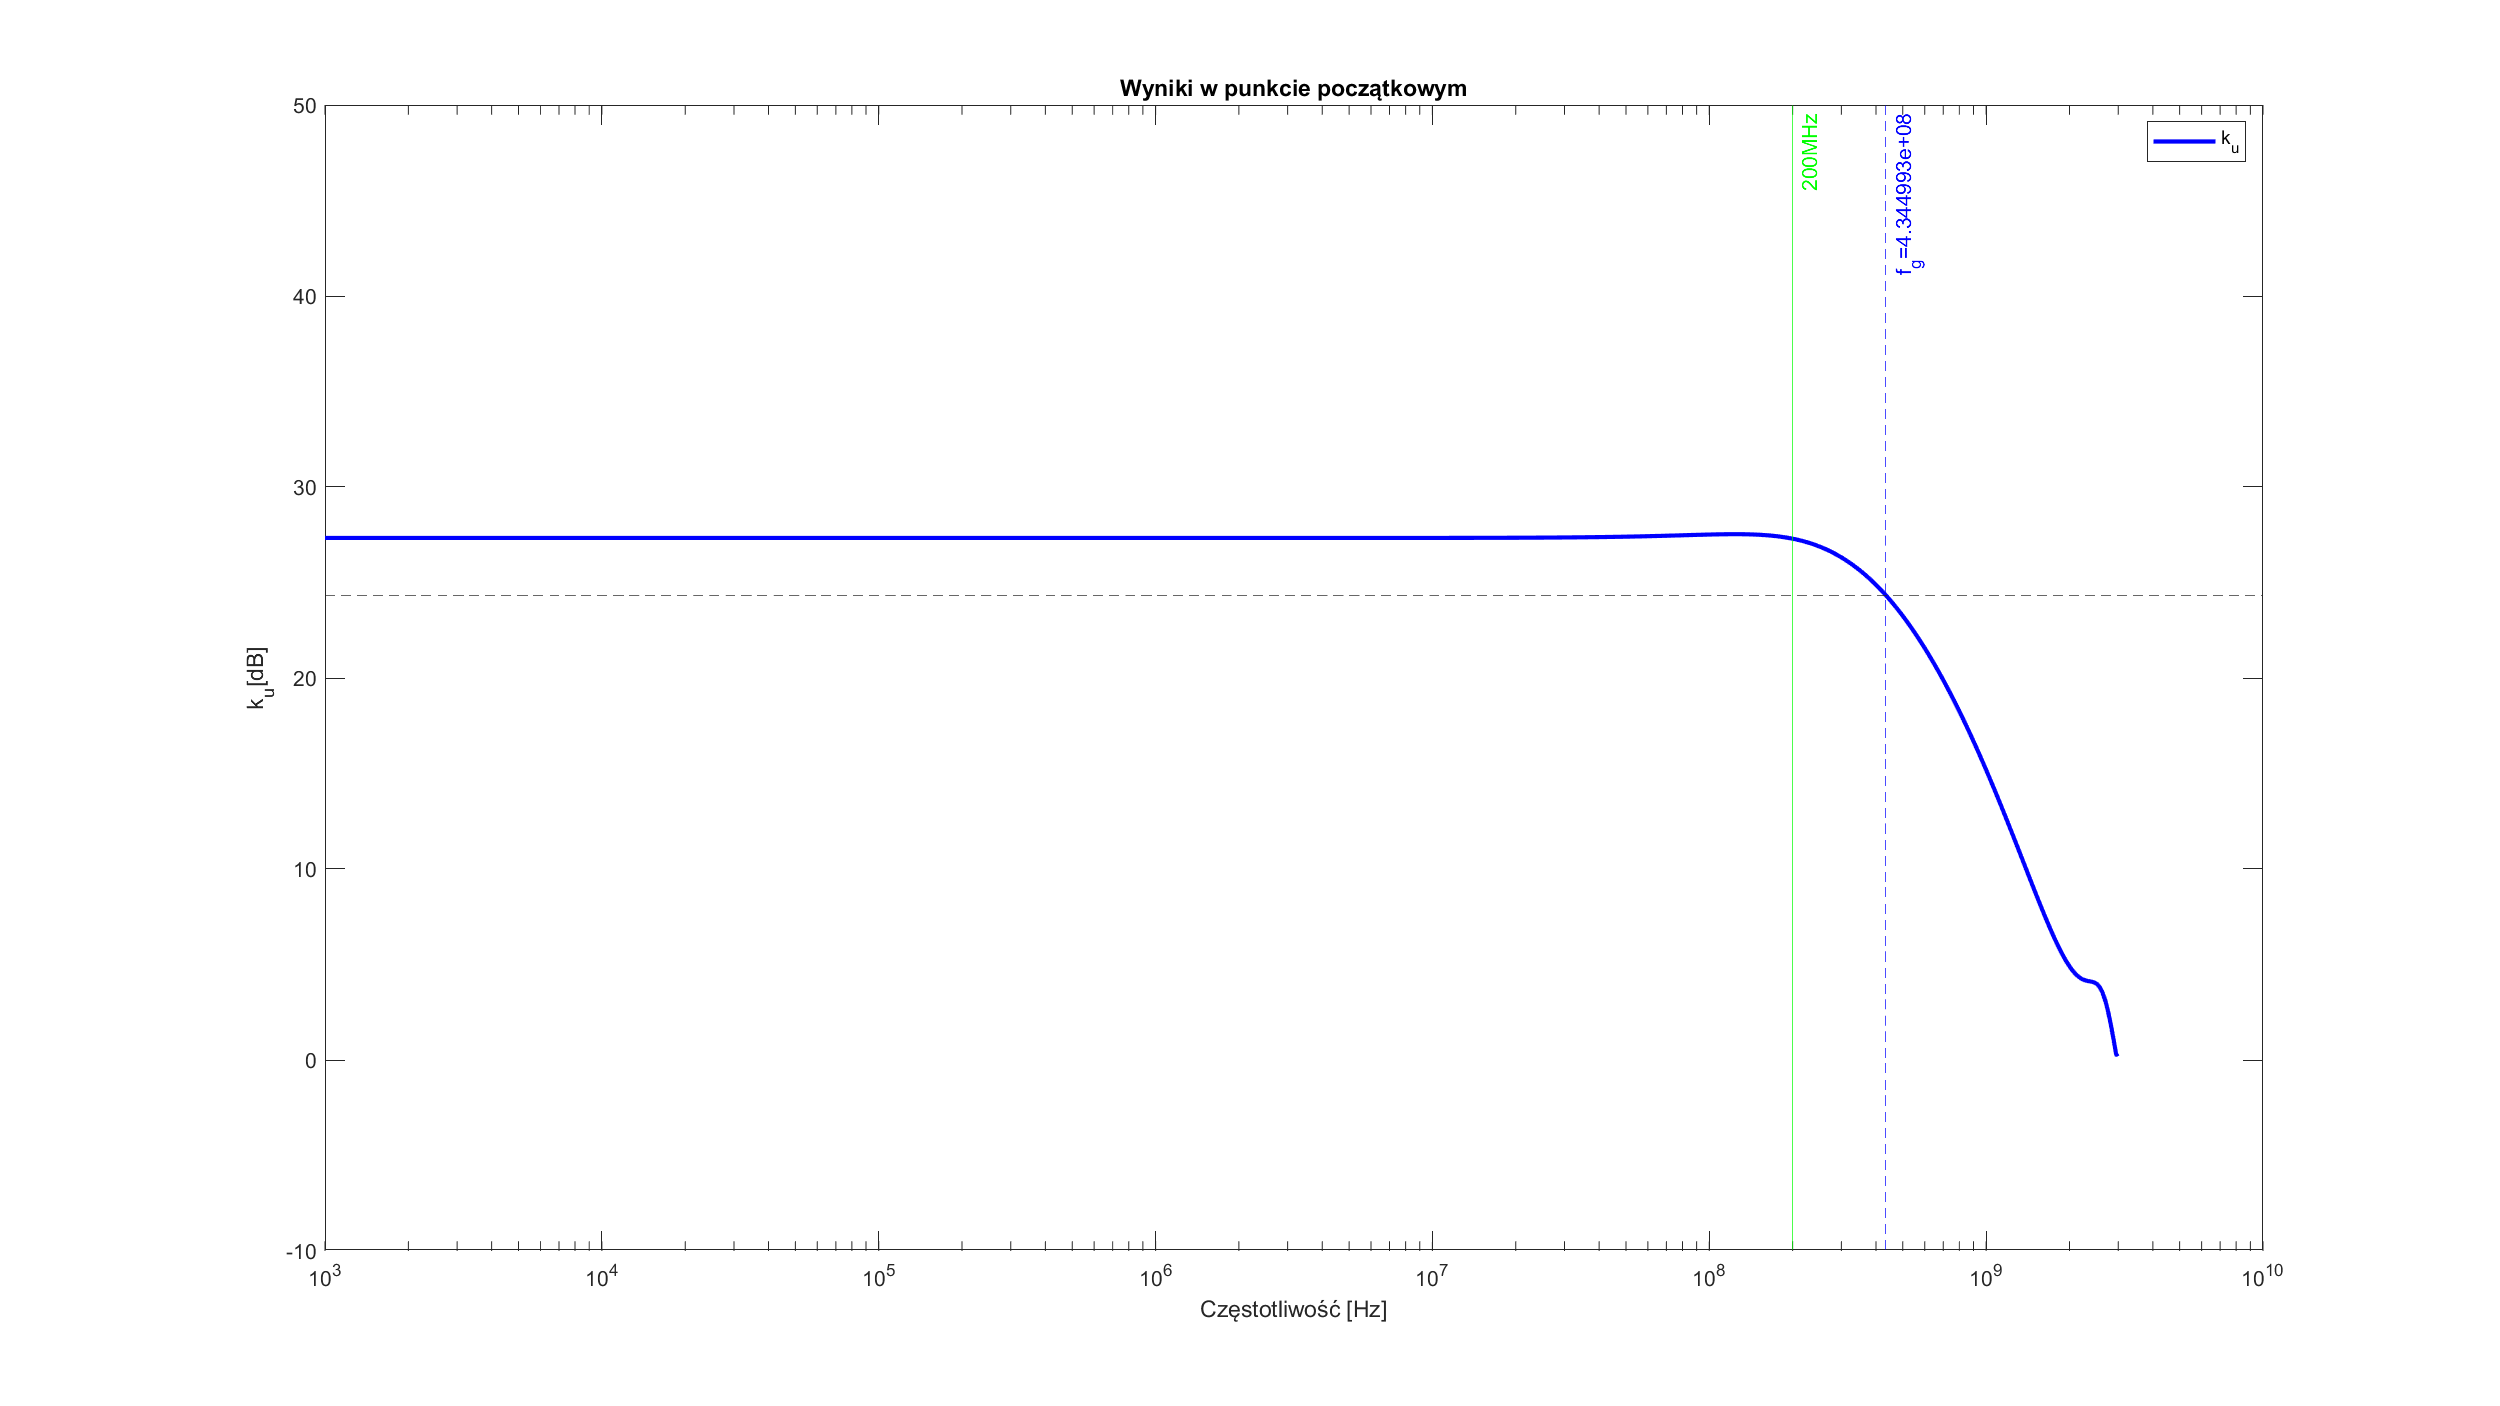
\includegraphics[width=25cm,height=15 cm]{graphics/starting_point.png}
        \centering
        \caption{Charakterystyka układu w punkcie startowym.}
    \end{figure}
\end{landscape}

\clearpage
\pagebreak
\begin{landscape}
    \begin{figure}[h]
        \vspace*{-2cm}
        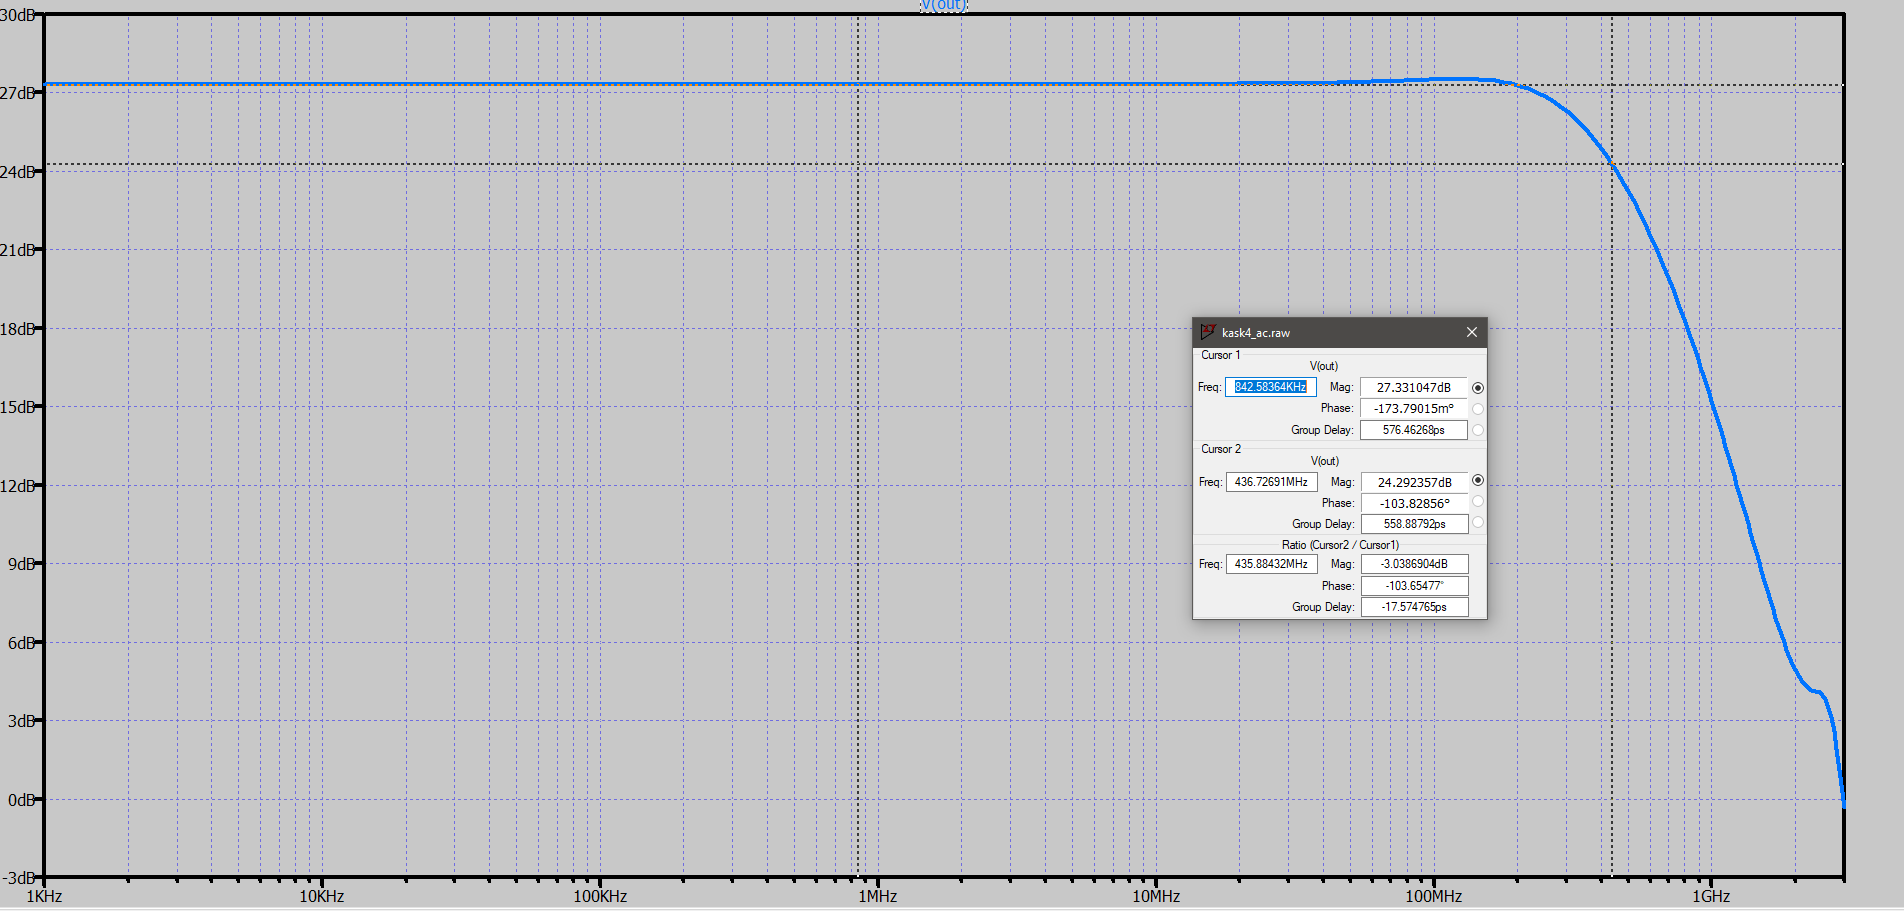
\includegraphics[width=20cm,height=10 cm]{graphics/starting_point_spice.png}
        \centering
        \caption{Charakterystyka układu w punkcie startowym (LTSpice).}
    \end{figure}
\end{landscape}

\pagebreak
\begin{landscape}
    \begin{figure}[h]
        \vspace*{-2cm}
        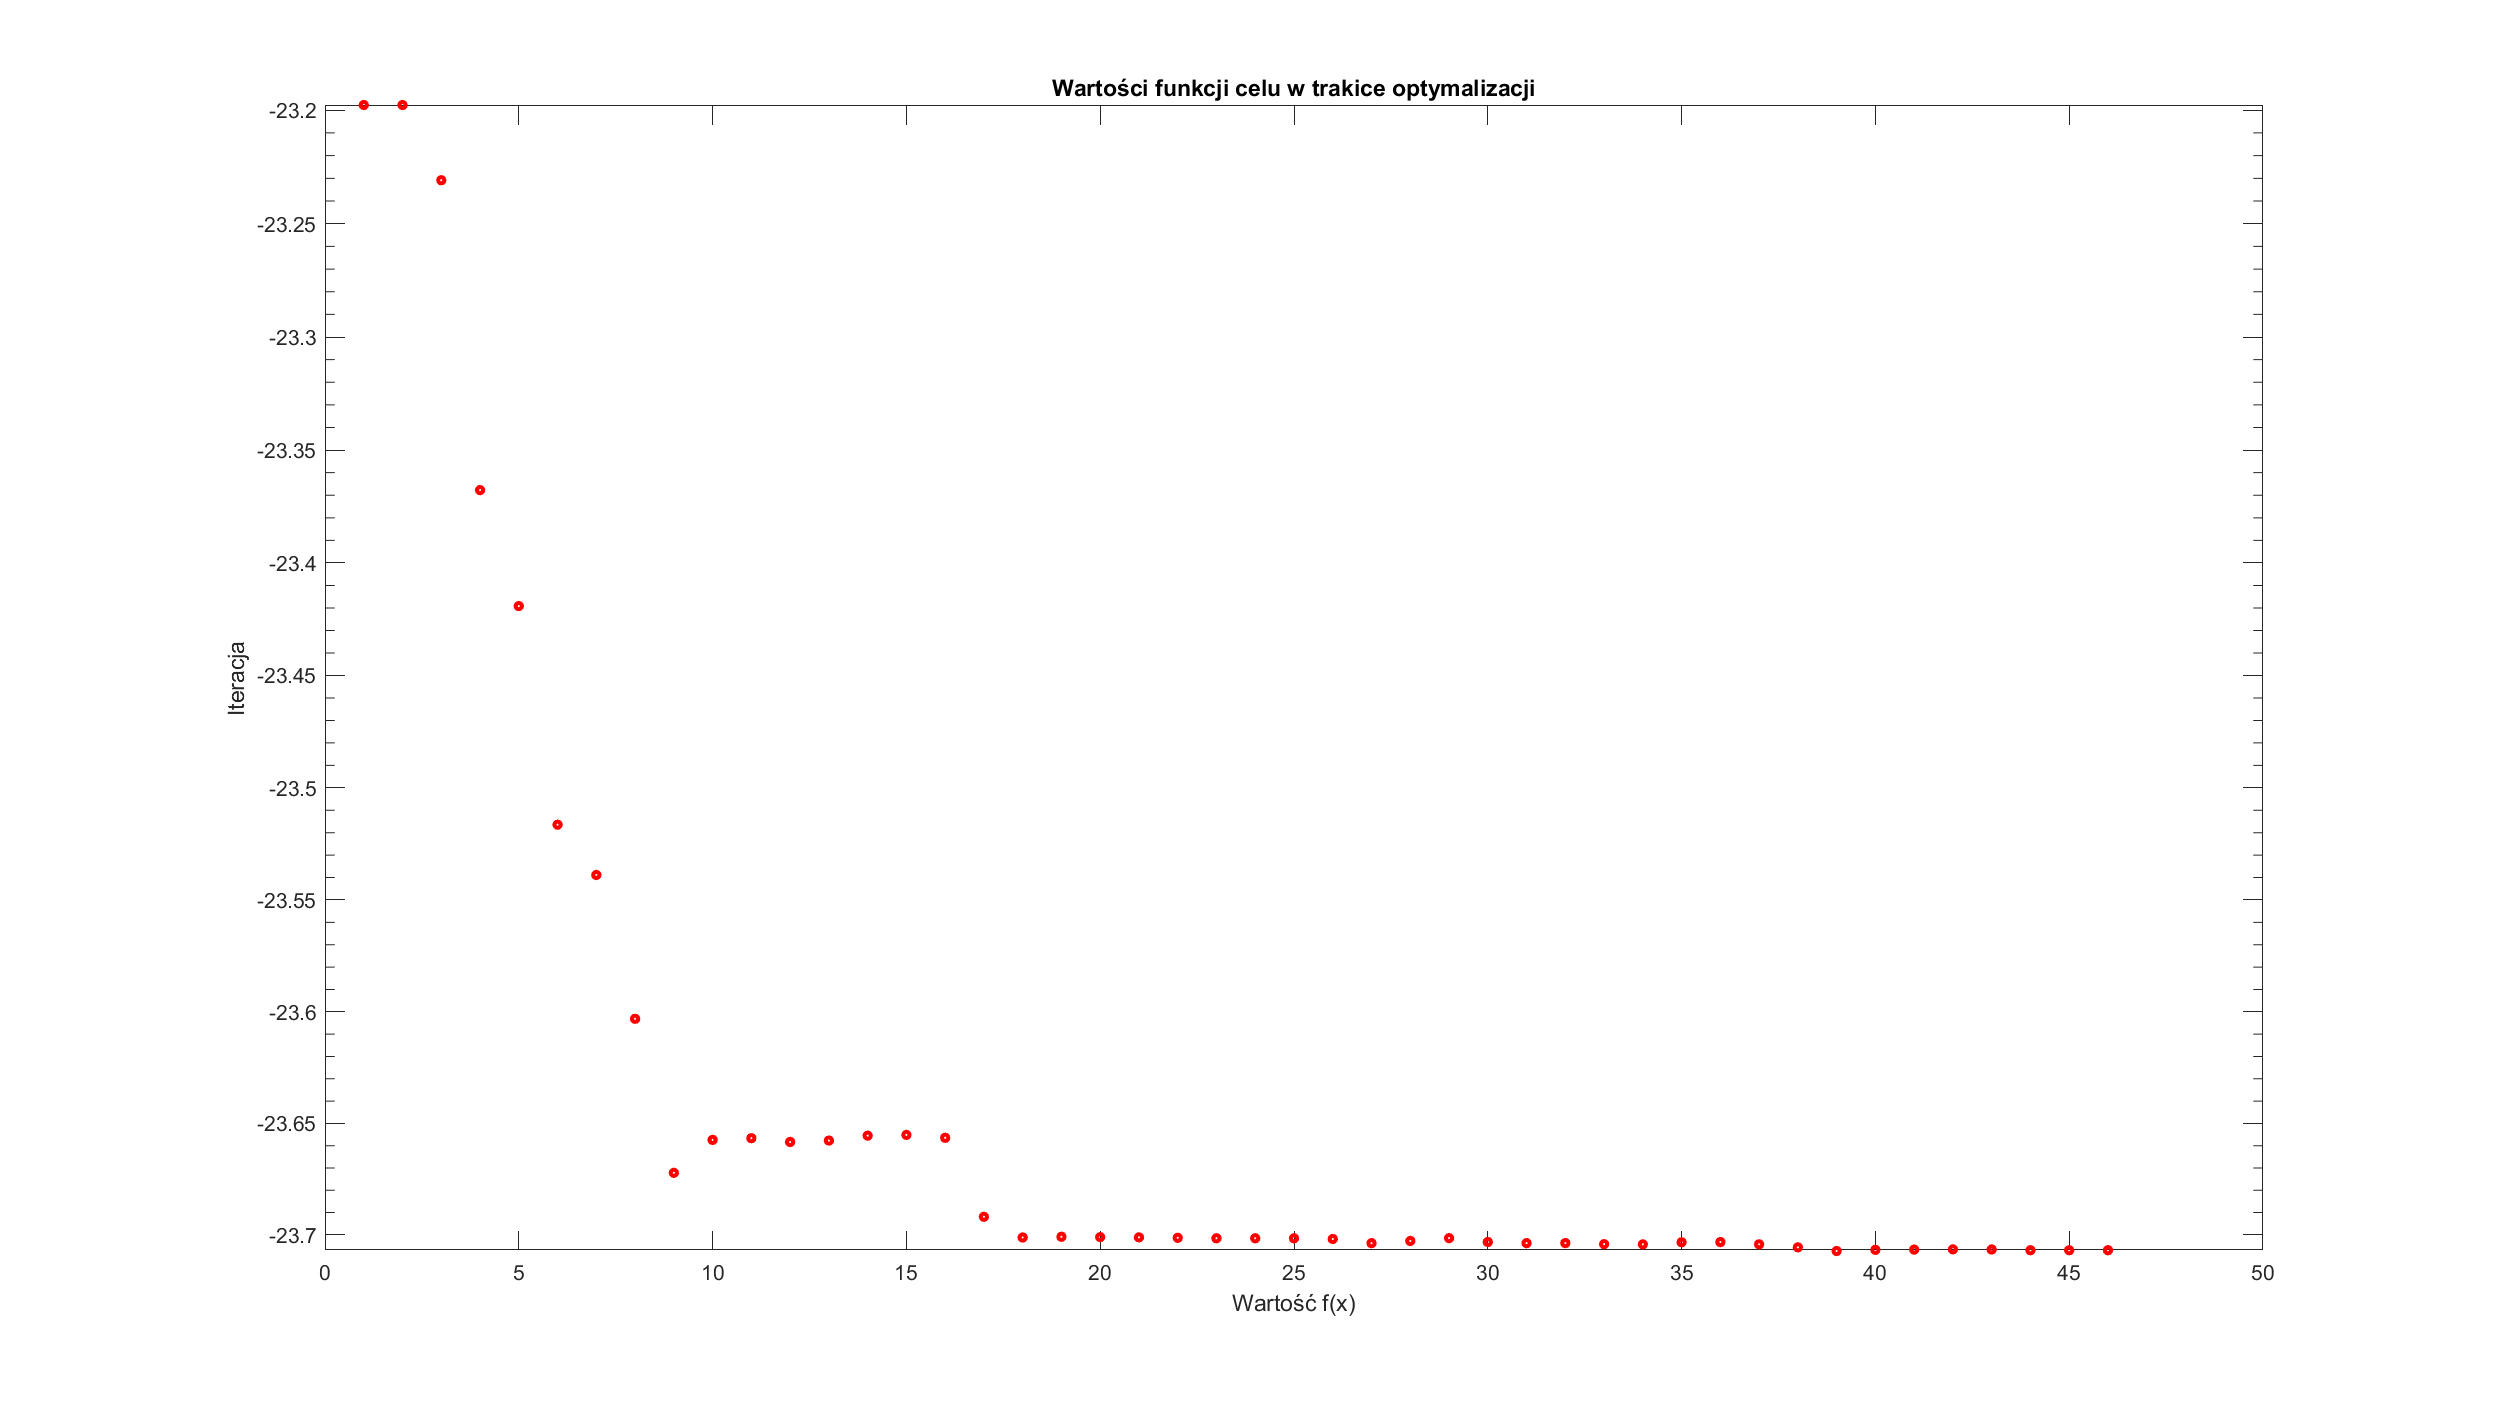
\includegraphics[width=25cm,height=15 cm]{graphics/fval.png}
        \centering
        \caption{Przebieg wartości funkcji celu.}
    \end{figure}
\end{landscape}

\pagebreak
\begin{landscape}
    \begin{figure}[h]
        \vspace*{-2cm}
        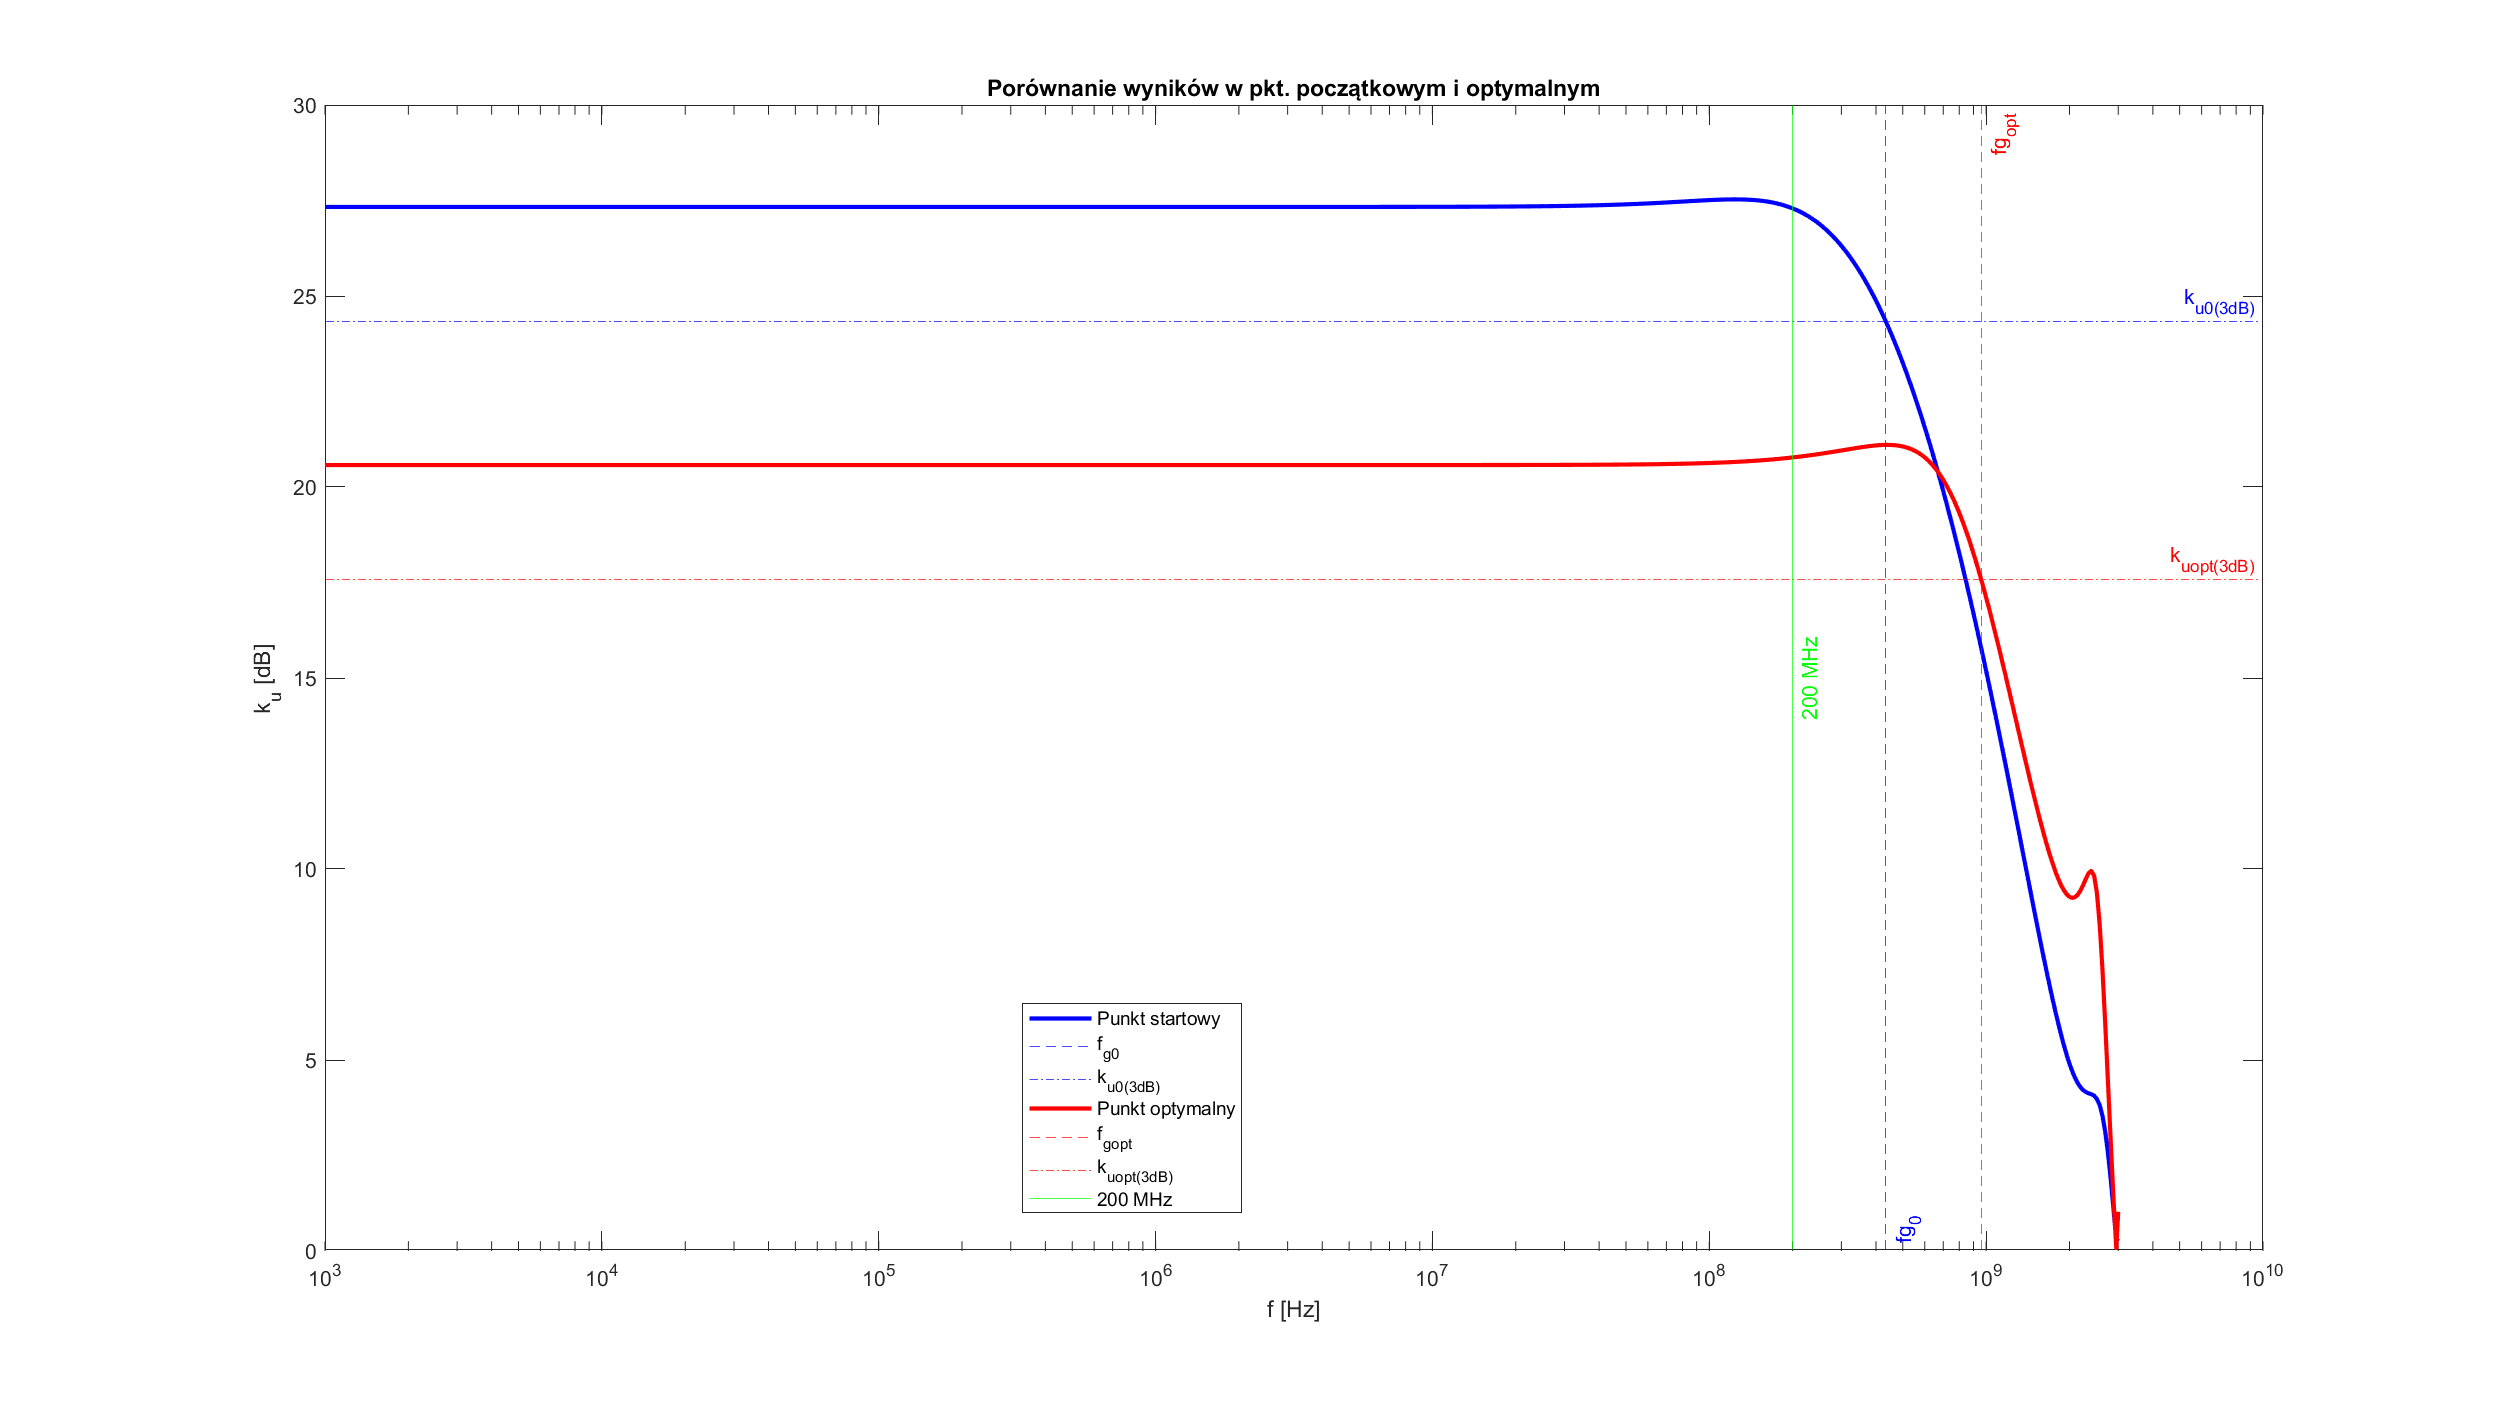
\includegraphics[width=25cm,height=15 cm]{graphics/comparison.png}
        \centering
        \caption{Porównanie wyników w punkcie optymalnym i startowym.}
    \end{figure}
\end{landscape}

\pagebreak
\begin{landscape}
    \begin{figure}[h]
        \vspace*{-2cm}
        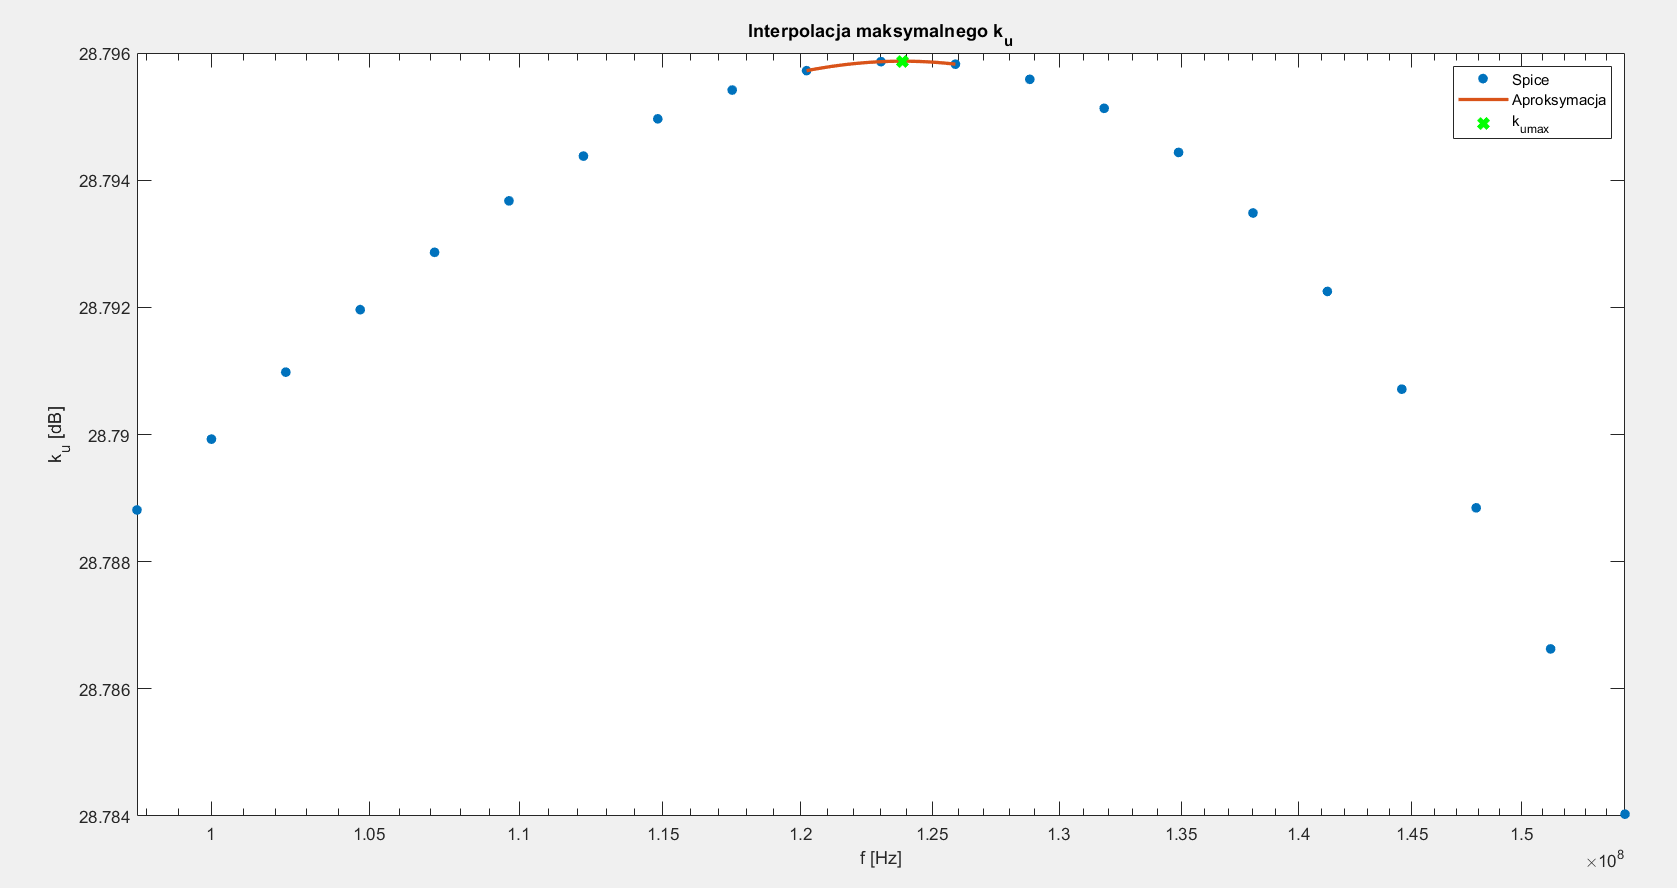
\includegraphics[width=20cm,height=10 cm]{graphics/max_ku_interp.png}
        \centering
        \caption{Interpolacja maksymalnego wzmocnienia.}
    \end{figure}
\end{landscape}

\pagebreak
\begin{landscape}
    \begin{figure}[h]
        \vspace*{-2cm}
        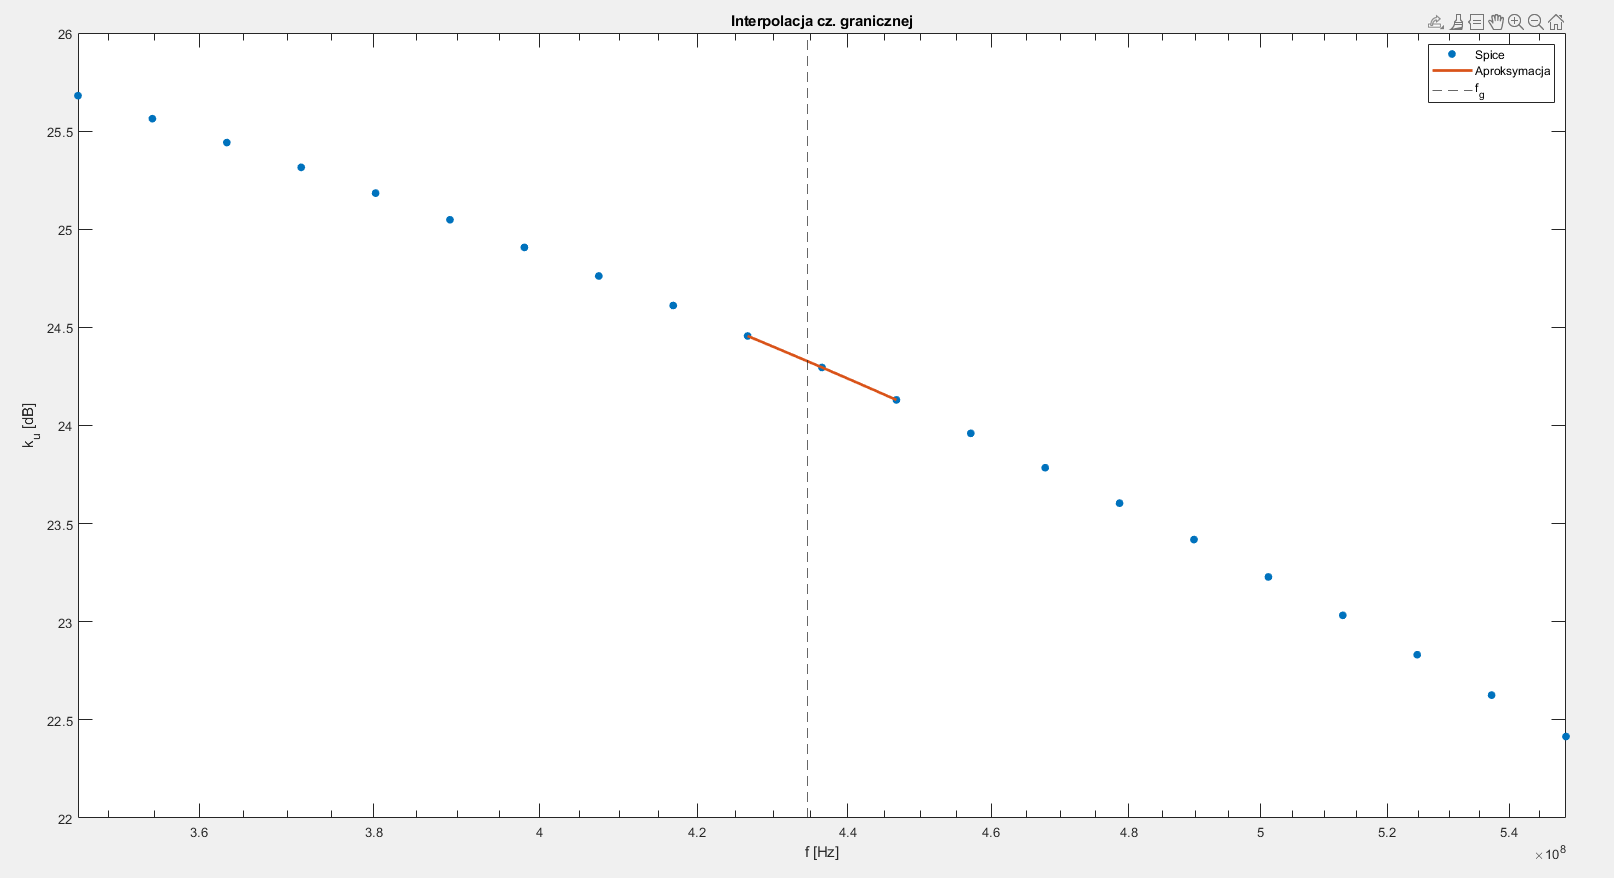
\includegraphics[width=20cm,height=10 cm]{graphics/fg_interp.png}
        \centering
        \caption{Interpolacja częstotliwości granicznej.}
    \end{figure}
\end{landscape}

\pagebreak
\begin{landscape}
    \begin{figure}[h]
        \vspace*{-2cm}
        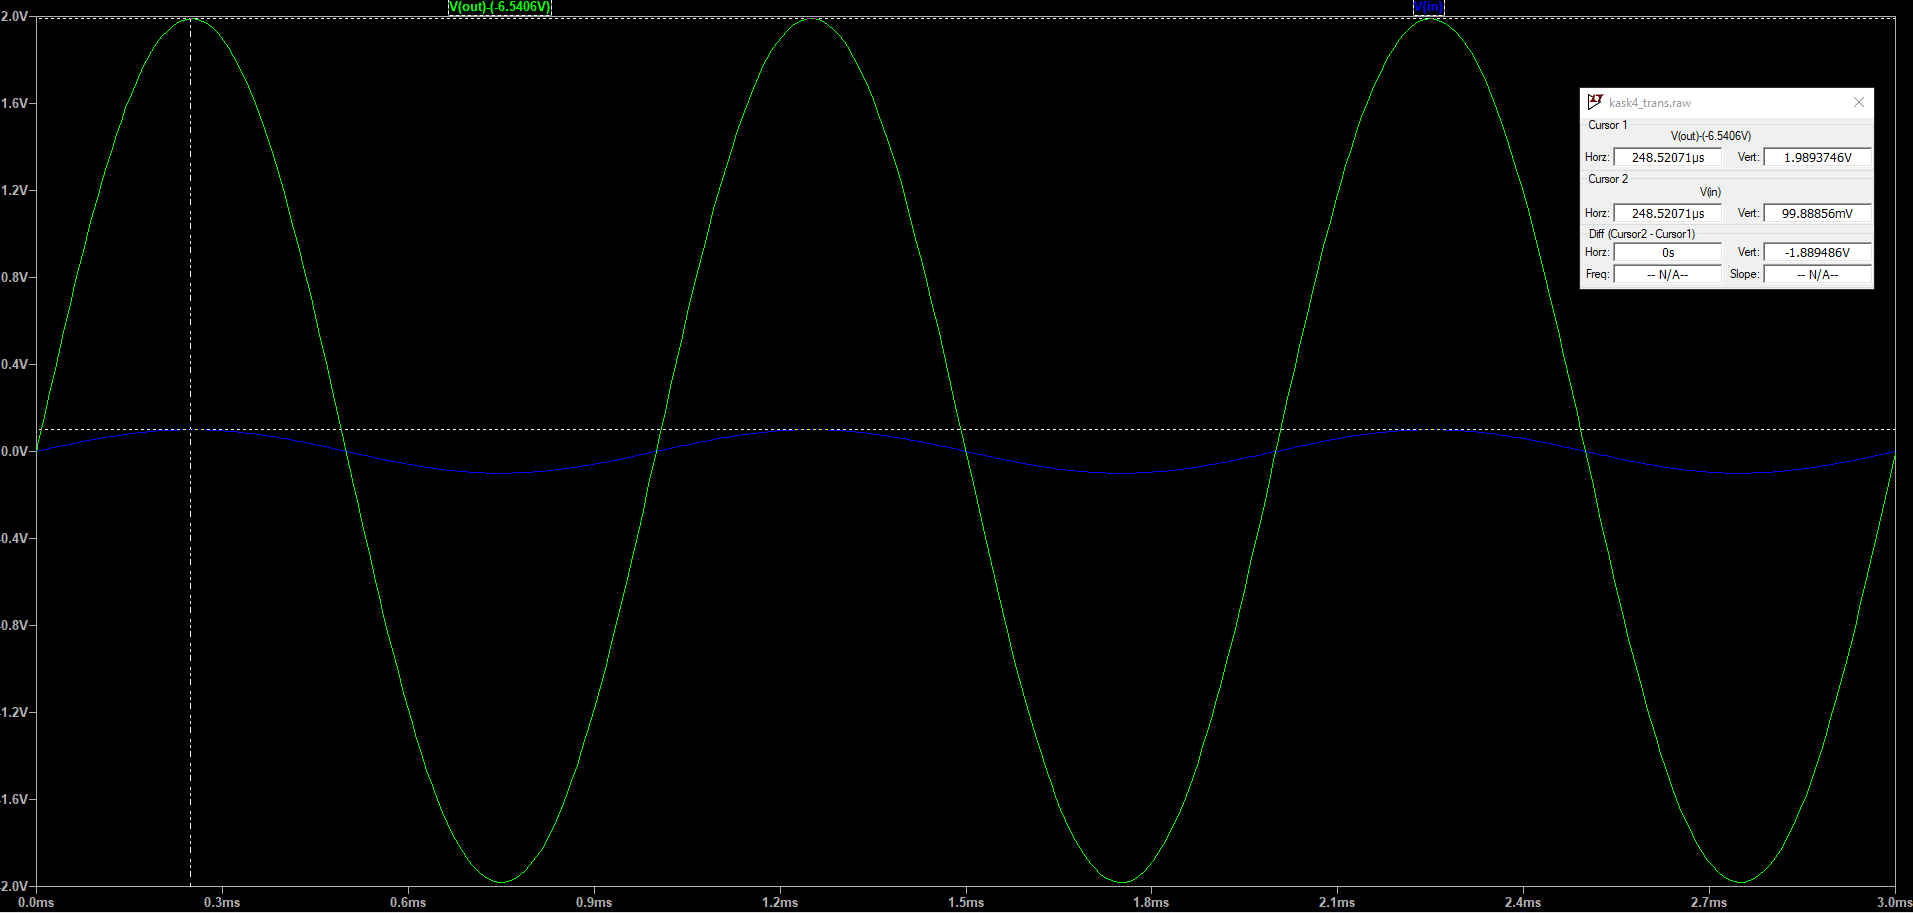
\includegraphics[width=20cm,height=10cm]{graphics/optim_tran.png}
        \centering
        \caption{Symulacja czasowa w pkt. optymalnym. Wzmacniacz wzmacnia.}
    \end{figure}
\end{landscape}

\pagebreak
\begin{landscape}
    \begin{figure}[h]
        \vspace*{-2cm}
        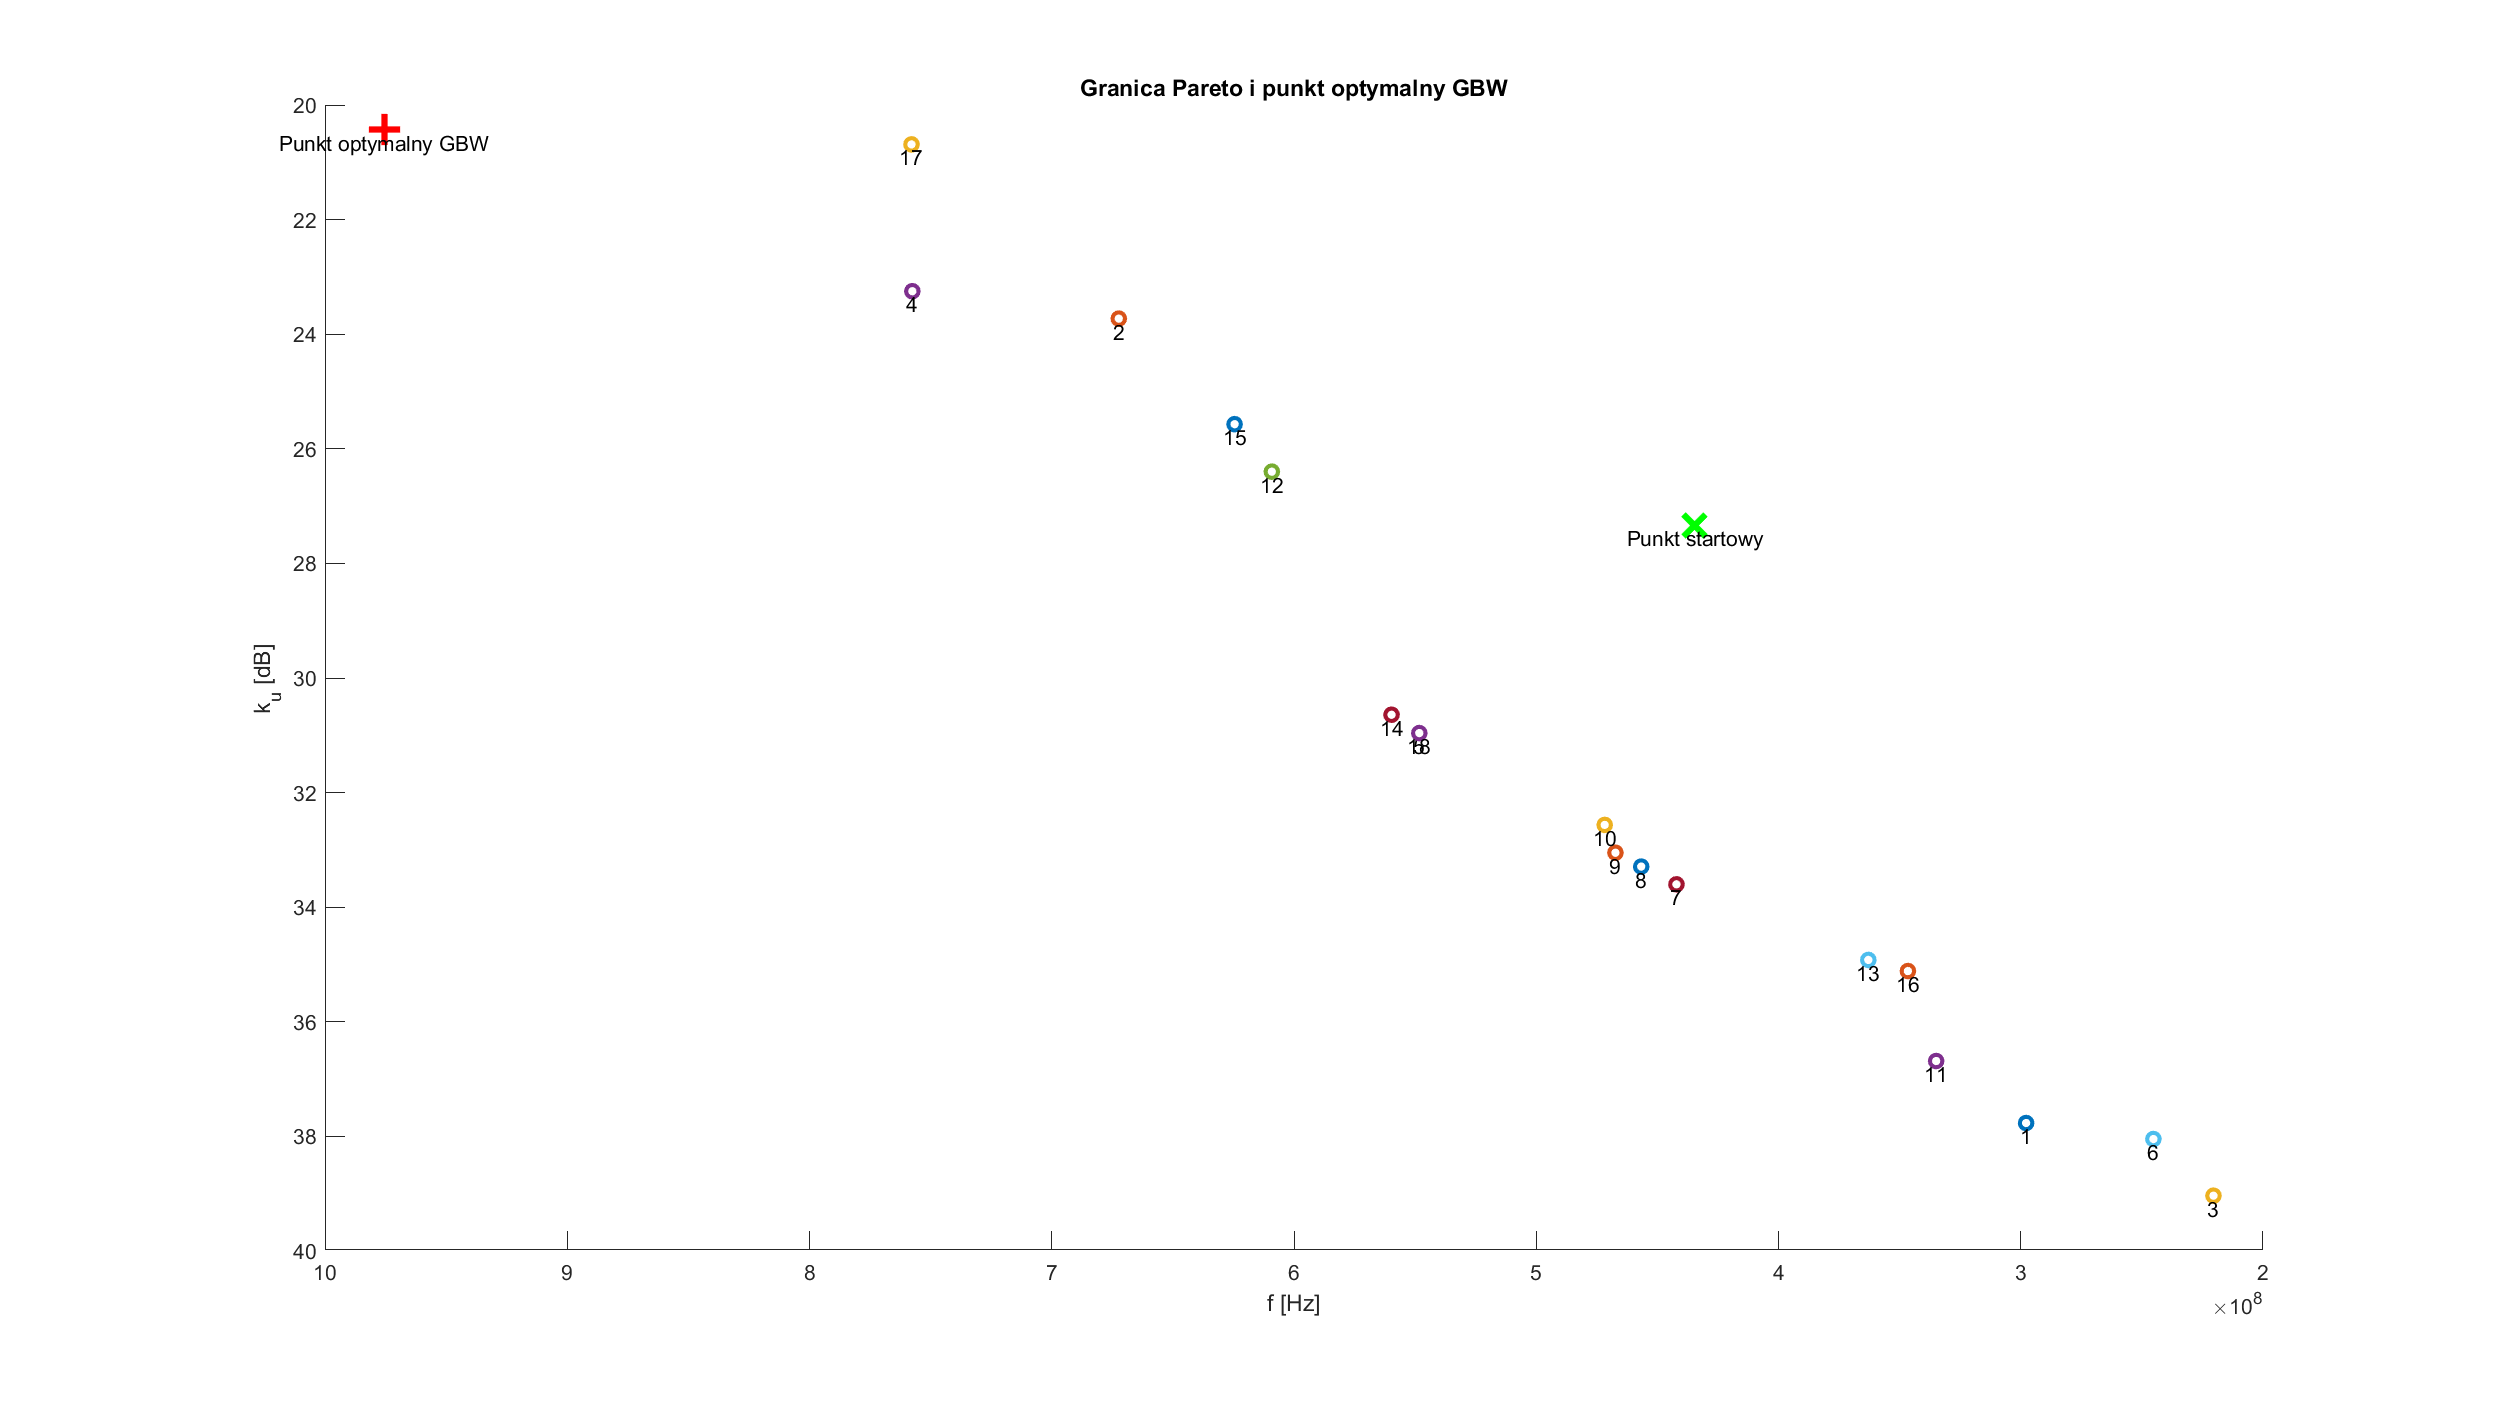
\includegraphics[width=20cm,height=10cm]{graphics/pareto.png}
        \centering
        \caption{Granica Pareto}
    \end{figure}
\end{landscape}

\end{document}



